% Heliyon research article. Compile from this directory:
%   pdflatex heliyon && pdflatex heliyon
\documentclass[preprint,12pt]{elsarticle}
\usepackage{amsmath,amssymb}
\usepackage{booktabs}
\usepackage{graphicx}
\usepackage{url}
\usepackage{multirow}
\journal{Heliyon}
\hyphenation{Fermi-GBM Batch-Norm iso-la-bil-ity}

% Auto-generated by src/lib/aria/paper_eval.ts. Do not edit by hand.
\newcommand{\AriaAcc}{90.0\pm0.6}
\newcommand{\RangeAcc}{43.1\pm6.0}
\newcommand{\NovelIso}{95.0\pm3.2}
\newcommand{\ComputeIso}{100.0\pm0.0}
\newcommand{\NovelAsCompute}{5.0\pm3.2}
\newcommand{\ExecPrec}{fp32}
\newcommand{\SensorIso}{77.5\pm0.6}
\newcommand{\AblFull}{90.0\pm0.6}
\newcommand{\AblChecksum}{62.4\pm0.2}
\newcommand{\AblPhysics}{53.5\pm0.0}
\newcommand{\AblMorph}{49.5\pm0.5}
\newcommand{\AblNoChecksum}{65.8\pm0.2}
\newcommand{\CompoundCompute}{100.0}
\newcommand{\CatalogTotal}{12981}
\newcommand{\CatalogGRB}{4375}
\newcommand{\CatalogTGF}{1658}
\newcommand{\CatalogSGR}{684}
\newcommand{\CatalogSflare}{2800}

% Auto-generated by experiments/gbm/make_realdata_tex.py from
% experiments/gbm/last_eval.json. Do not edit by hand.
\newcommand{\RealCubes}{100}
\newcommand{\RealPerClass}{25}
\newcommand{\RealTrials}{180}
\newcommand{\RealSeeds}{5}
\newcommand{\RealEvalSeed}{123}
\newcommand{\RealAriaAcc}{74.4}
\newcommand{\RealAriaAccPM}{74.4\pm0.0}
\newcommand{\RealRangeAcc}{43.3}
\newcommand{\RealRangeAccPM}{43.3\pm0.0}
\newcommand{\RealComputeIso}{100.0}
\newcommand{\RealComputeIsoPM}{100.0\pm0.0}
\newcommand{\RealSensorIso}{60.0}
\newcommand{\RealSensorIsoPM}{60.0\pm0.0}
\newcommand{\RealNovelIso}{0.0}
\newcommand{\RealNovelIsoPM}{0.0\pm0.0}
\newcommand{\RealNovelAsCompute}{0.0}
\newcommand{\RealNovelAsComputePM}{0.0\pm0.0}
\newcommand{\RealEnergyCompute}{27.5}
\newcommand{\RealEnergyComputePM}{27.5\pm0.0}
\newcommand{\RealEnergyNovel}{0.0}
\newcommand{\RealEnergyNovelPM}{0.0\pm0.0}

% Auto-generated by make_check_figures.py. Do not edit by hand.
\newcommand{\CalAccThirtyTwo}{90.0 $\pm$ 0.6}
\newcommand{\CalNovCompThirtyTwo}{5.0 $\pm$ 3.2}
\newcommand{\CalCompThirtyTwo}{100.0 $\pm$ 0.0}
\newcommand{\CalMildThirtyTwo}{100.0 $\pm$ 0.0}
\newcommand{\CalAucThirtyTwo}{1.000}
\newcommand{\CalAccSixteen}{86.3 $\pm$ 1.2}
\newcommand{\CalNovCompSixteen}{4.4 $\pm$ 6.2}
\newcommand{\CalCompSixteen}{84.2 $\pm$ 5.0}
\newcommand{\CalMildSixteen}{76.1 $\pm$ 6.0}
\newcommand{\CalAucSixteen}{0.929}
\newcommand{\BndAccThirtyTwo}{90.8 $\pm$ 0.2}
\newcommand{\BndNovCompThirtyTwo}{0.0 $\pm$ 0.0}
\newcommand{\BndCompThirtyTwo}{100.0 $\pm$ 0.0}
\newcommand{\BndMildThirtyTwo}{100.0 $\pm$ 0.0}
\newcommand{\BndAucThirtyTwo}{1.000}
\newcommand{\BndAccSixteen}{77.4 $\pm$ 0.3}
\newcommand{\BndNovCompSixteen}{0.0 $\pm$ 0.0}
\newcommand{\BndCompSixteen}{46.1 $\pm$ 1.0}
\newcommand{\BndMildSixteen}{15.6 $\pm$ 1.4}
\newcommand{\BndAucSixteen}{0.964}
\newcommand{\BoundWorstRatio}{0.15}
\newcommand{\BoundInputs}{40{,}000}
\newcommand{\BoundMaxSigma}{1000}
\newcommand{\RealBndSensEight}{70.8}
\newcommand{\RealCalSensEight}{58.3}
\newcommand{\RealCalNovCompTwelve}{8.3}
\newcommand{\RealBndCompSixteenEight}{79.2}
\newcommand{\RealBndCompSixteenTwelve}{91.7}
\newcommand{\RealBndCompSixteenTwentyFive}{95.0}

% Auto-generated by src/lib/aria/extra_eval.ts. Do not edit by hand.
\newcommand{\CvAcc}{77.2\pm2.7}
\newcommand{\CvNovel}{0.0\pm0.0}
\newcommand{\CvNovelComp}{0.0\pm0.0}
\newcommand{\CvComp}{100.0\pm0.0}
\newcommand{\CvSens}{65.3\pm7.5}
\newcommand{\CvAllAcc}{77.2\pm2.7}
\newcommand{\CvAllSens}{65.3\pm7.5}
\newcommand{\CvAllComp}{100.0\pm0.0}
\newcommand{\SplitABAcc}{77.7\pm0.0}
\newcommand{\SplitABSens}{66.7\pm0.0}
\newcommand{\SplitABComp}{100.0\pm0.0}
\newcommand{\SplitABNovC}{0.0\pm0.0}
\newcommand{\SplitBAAcc}{80.0\pm0.0}
\newcommand{\SplitBASens}{72.2\pm0.0}
\newcommand{\SplitBAComp}{100.0\pm0.0}
\newcommand{\SplitBANovC}{0.0\pm0.0}
\newcommand{\MildComp}{100.0\pm0.0}
\newcommand{\AllSens}{69.3\pm0.0}
\newcommand{\AllAcc}{78.8\pm0.0}
\newcommand{\AllComp}{100.0\pm0.0}
\newcommand{\BothSig}{79.2\pm3.1}
\newcommand{\ArithOnly}{20.7\pm3.1}
\newcommand{\MultiRate}{79.2\pm3.1}
\newcommand{\SimSpikeSens}{86.7\pm0.7}
\newcommand{\SimHeadSens}{77.5\pm0.6}
\newcommand{\SimSpikeKnown}{9.4\pm0.4}
\newcommand{\SimHeadKnown}{9.3\pm0.0}
\newcommand{\SimSpikeAcc}{92.2\pm0.6}
\newcommand{\RealSpikeSens}{60.0\pm0.0}
\newcommand{\RealSpikeKnown}{2.7\pm0.0}
\newcommand{\RealSpikeAcc}{74.4\pm0.0}
\newcommand{\RealSpikeNovS}{0.0\pm0.0}
\newcommand{\TgfAsKnown}{100.0}


\begin{document}

\begin{frontmatter}

\title{Which cause is it? Selectively blind residuals for isolating compute faults, sensor glitches, and novel classes in multi-detector neural inference}

\author[cse]{Haripriya S.\corref{cor}}
\author[ece]{Suhasini S.}
\affiliation[cse]{organization={School of Computer Science and Engineering, Vellore Institute of Technology},
            addressline={Chennai 600127},
            country={India}}
\affiliation[ece]{organization={School of Electronics Engineering, Vellore Institute of Technology},
            addressline={Chennai 600127},
            country={India}}
\cortext[cor]{Corresponding author.}
\ead{haripriya.subbiah@gmail.com}

\begin{abstract}
A classifier that watches a redundant detector array can be wrong for four mechanistically different reasons: the source is a class the network was trained on, the source is a class it has never seen, one detector glitched, or the arithmetic inside the classifier was silently corrupted. Open-set scores, silent-data-corruption monitors, and range checks all read activation magnitude, so a new physical class and a flipped weight can raise the same alarm. This paper specifies a four-symbol isolability dictionary, with symbols for a known class, a novel class, a sensor fault, and a compute fault, and four residuals that are each blind to at least one symbol. A physics residual compares detectors and does not read the weights. A checksum of the linear head does not read the sky. A morphology residual is computed on the shared profile, so a corrupt head cannot invent a discovery. The decision is a lookup that reads the checksum first. On an eight-detector Fermi Gamma-ray Burst Monitor simulator, five training seeds give $\AriaAcc\%$ four-way accuracy, against $\RangeAcc\%$ for a range check. Held-out flashes are called novel in $\NovelIso\%$ of trials and a compute fault in $\NovelAsCompute\%$. A rounding-error bound removes that leak at 32-bit precision. A fusion trained on labeled residuals reaches 96.5\% and calls no flash a compute fault. On a spike plus a bit-flip it usually names the sensor, while the lookup names compute. On \RealCubes{} public continuous-time triggers, bit-flips stay isolated and no flash is called novel. A second disjoint draw of \RealCubes{} triggers keeps both of those results. Sensor isolation does not: it is 65\% in one direction and 7.5\% in the other. At 1\,ms, 23 of 24 flashes leave a burst-only cloud, and the lookup calls them sensor.
\end{abstract}

\begin{highlights}
\item Four residuals, each blind to at least one of four causes.
\item The lookup reads the checksum first.
\item Simulator accuracy is 90.0\%; a range check reaches 43.1\%.
\item A rounding bound stops false compute calls at 32-bit precision.
\item At 1 ms, morphology separates flashes; the lookup says sensor.
\end{highlights}

\begin{keyword}
silent data corruption \sep open-set recognition \sep Fermi GBM \sep structured residuals \sep isolability \sep algorithm-based fault tolerance \sep embedded neural networks
\end{keyword}

\begin{graphicalabstract}
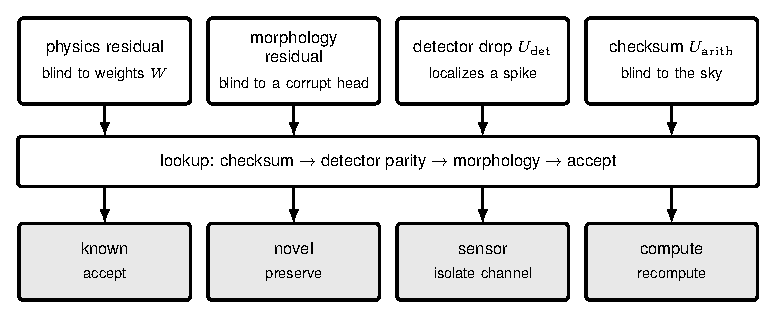
\includegraphics[width=0.92\textwidth]{fig_method.pdf}
\end{graphicalabstract}

\end{frontmatter}

\section{Introduction}

Deployed neural networks fail for reasons that call for opposite responses. If a wearable, a rover, or an onboard gamma-ray monitor sees an unusual activation, the operator may need to accept a known event, preserve a possible discovery, isolate a bad sensor, or recompute a flipped weight. Treating those four outcomes as one anomaly is not a small labeling error. Adapting a model to a bit-flip poisons a good network. Discarding a new physical class as a glitch throws away the event the instrument was built to catch.

The Fermi Gamma-ray Burst Monitor (GBM) is a concrete instance. Twelve sodium iodide (NaI) detectors and two bismuth germanate (BGO) detectors observe the unocculted sky. Catalogued triggers include gamma-ray bursts (GRBs), solar flares, magnetar bursts (SGRs), terrestrial gamma-ray flashes (TGFs), and local and distant particle events~\cite{meegan2009,vonkienlin2020,bhat2016,roberts2018,briggs2013}. Public classifiers already sort known classes and flag outliers~\cite{john2025}. They do not treat a corrupted matrix multiply as a cause, and they do not have to: ground pipelines assume correct arithmetic. Onboard or edge inference cannot. Silent data corruption is documented in production fleets~\cite{dixit2021,hochschild2021,dixit2022}, and soft errors can propagate to neural-network outputs depending on data types and layers~\cite{li2017,reagen2018}.

The closest reliability papers still collapse causes. Gavarini and colleagues use open-set scores as fault detectors~\cite{gavarini2022}. ProGIP distinguishes in-distribution, out-of-distribution (OOD), and high-order bit-flips with range checks on gradient-based OOD scores~\cite{progip2025}. Dr.~DNA and related activation monitors flag silent data corruption (SDC) from the shape of neuron histograms~\cite{drdna2024,geissler2023}. ReAct showed that OOD inputs already produce extreme activations~\cite{react2021}, the same symptom high-order bit-flips produce. Classical isolability names sensor, process, and actuator faults~\cite{gertler1990,venkatasubramanian2003,isermann2005}. It has no symbol for a new astrophysical class. Fermi pipelines already veto single-detector phosphorescent spikes~\cite{paciesas2012,goldstein2019,perera2025}. They do not close that veto with an input-invariant execution checksum.

The contribution is a dictionary, not a new optimizer or a new sequential test:
\begin{itemize}
\item four causes, known, novel, sensor, and compute, with mutually exclusive operational responses;
\item four residuals that are selectively blind, so the binary pattern names the cause under a single-fault assumption;
\item a public evaluation, with no graphics processing unit, against OOD-as-fault and range-check baselines, including the places the dictionary fails.
\end{itemize}

The limit is stated up front. The five-seed four-way tables use a cosine-response, Poisson eight-detector simulator whose class morphologies follow GBM families. Counts from the High Energy Astrophysics Science Archive Research Center (HEASARC) catalog are real. Section~\ref{sec:real} repeats the same lookup on \RealCubes{} public continuous-time (CTIME) cubes. Section~\ref{sec:tte} scores the same families as time-tagged events. A burst-only distance at 1\,ms separates most flashes. The four-way lookup on those files calls the flashes a sensor fault. Software bit-flips are radiation-like, not a beam test. Section~\ref{sec:extra} then measures four things the headline protocol leaves open: whether the known-class numbers survive a split, why the novel symbol is empty on CTIME, whether a short-window spike score repairs sensor isolation, and how often two simultaneous faults light two residuals at once.

\section{Related work}
\label{sec:related}

Table~\ref{tab:compare} places the closest methods against the four causes and against the two structural properties this paper uses. A ``part'' entry means the method touches that column only inside an undifferentiated score. The isolability claim holds under the single-fault assumption only.

\begin{table*}[t]
\caption{Comparison of closely related methods. OOD: open-set or out-of-distribution detection. Compute: silent arithmetic or weight corruption. Sensor: a sensor fault is separated from the sky. Novel kept: ``new class'' is returned as a non-fault outcome. Physics: a physics or plant-model residual is used. Isolability: the paper argues that a residual signature identifies the cause.}
\label{tab:compare}
\centering
\footnotesize
\setlength{\tabcolsep}{4pt}
\resizebox{\textwidth}{!}{%
\begin{tabular}{lcccccc}
\toprule
Method & OOD & Compute & Sensor & Novel kept & Physics & Isolability \\
\midrule
MSP, energy, ODIN~\cite{hendrycks2017,liu2020,liang2018} & Yes & No & No & No & No & No \\
Mahalanobis, G-ODIN, ViM~\cite{lee2018,hsu2020,wang2022} & Yes & No & No & No & No & No \\
OpenMax, Scheirer, Vaze~\cite{scheirer2013,bendale2016,vaze2022} & Yes & No & No & Part. & No & No \\
Gavarini~\cite{gavarini2022} & Yes & Part. & No & No & No & No \\
ProGIP~\cite{progip2025} & Yes & Yes & No & Part. & No & No \\
Dr.\ DNA~\cite{drdna2024} & No & Yes & No & No & No & No \\
Geissler, FACER~\cite{geissler2023,schorn2020} & No & Part. & No & No & No & No \\
BLINK~\cite{blink2026} & No & Yes & No & No & No & No \\
FT-CNN, Huang--Abraham~\cite{zhao2021,huang1984} & No & Yes & No & No & No & No \\
Ares, Li and colleagues~\cite{reagen2018,li2017} & No & Yes & No & No & No & No \\
Dixit and colleagues~\cite{dixit2021} & No & Yes & No & No & No & No \\
Gertler--Singer, Isermann~\cite{gertler1990,isermann2005} & No & No & Yes & No & Yes & Yes \\
John and colleagues~\cite{john2025} & Part. & No & No & Part. & No & No \\
Perera and colleagues~\cite{perera2025} & No & No & Part. & No & Part. & No \\
\midrule
This work & Yes & Yes & Yes & Yes & Yes & Yes \\
\bottomrule
\end{tabular}}
\end{table*}

\subsection{Open-set scores used as fault detectors}

Maximum softmax probability~\cite{hendrycks2017}, the energy score~\cite{liu2020}, ODIN~\cite{liang2018}, the Mahalanobis score~\cite{lee2018}, generalized ODIN~\cite{hsu2020}, and virtual-logit matching~\cite{wang2022} reduce a surprising input to a reject bit. OpenMax~\cite{bendale2016} and the open-set line that begins with Scheirer and colleagues~\cite{scheirer2013,geng2021} add an explicit unknown class. Vaze and colleagues showed that a strong closed-set classifier, scored by its maximum logit, is already a competitive open-set detector~\cite{vaze2022}. Gavarini and colleagues then treat those bits as fault detectors~\cite{gavarini2022}. That is the failure mode this work exists to prevent: a held-out TGF is supposed to look unusual. An OOD alarm cannot say whether to preserve the event or recompute the product. Selective classification with OOD likewise accepts or rejects; it does not name compute faults~\cite{sirc2022,narasimhan2024}. Surveys of deep anomaly detection document the same collapse of ``unusual'' into one class~\cite{ruff2021}. Benchmarks such as OpenOOD compare detectors inside that one class~\cite{yang2022}.

\subsection{In-distribution, OOD, and fault in magnitude space}

ProGIP is the closest prior paper~\cite{progip2025}. It places range checkers on gradient-based input perturbation so that in-distribution inputs, OOD inputs, and high-order bit-flips can be separated in software. The checkers still operate on gradients and confidence scores. ReAct already showed that OOD inputs drive activations into the same extreme range that high-order flips occupy~\cite{react2021}. Range is a useful heuristic. It is not an identifiability argument, and it does not use instrument physics or a separate sensor symbol.

\subsection{Activation signatures for silent data corruption}

Dr.~DNA extracts SDC signatures from neuron-activation histograms~\cite{drdna2024}. Quantile-marker monitors flag corruption ``originating either from hardware memory faults or input corruptions'' as one class~\cite{geissler2023}. FACER compresses intermediate features and likewise treats hardware faults and unusual inputs as one anomaly~\cite{schorn2020}. BLINK compares live batch-normalization statistics with frozen running statistics~\cite{blink2026}. Fault-injection tools measure how often a flip changes an output~\cite{li2017,reagen2018,pytorchfi2020}. None of these methods is built to return ``this is a new class'' as a non-fault outcome.

\subsection{Structured residuals and checksums}

Gertler and Singer isolate faults with structured parity equations~\cite{gertler1990}. The process-monitoring surveys use the same idea: a residual is useful when it is insensitive to one fault and sensitive to another~\cite{venkatasubramanian2003,isermann2005,chen1999}. The dictionary in that literature is sensor, process, and actuator. Algorithm-based fault tolerance, beginning with Huang and Abraham~\cite{huang1984} and continued by FT-CNN~\cite{zhao2021}, detects a matrix-multiply error independently of the input. This paper uses a row-sum checksum as one residual. The checksum is not the contribution. Intensity-guided and approximate checksums decide where, or how loosely, to check~\cite{kosaian2021,approxabft2023}. They do not name discovery. The rounding analysis below uses the standard model of floating-point error~\cite{higham2002,ieee754}.

\subsection{Fermi-GBM classification and vetoes}

John and colleagues train convolutional-recurrent classifiers on public GBM triggers and flag events outside the four trained classes as outliers~\cite{john2025}. Flight software already requires a rate increase in two or more NaI detectors before it triggers~\cite{meegan2009}, which suppresses artefacts that appear in only one detector~\cite{paciesas2012}. Ground localization compares the relative rates of the NaI detectors~\cite{goldstein2020,connaughton2015}. Perera and colleagues search all GBM detectors with a Poisson matched filter and estimate whether a candidate is cosmological, terrestrial, or solar~\cite{perera2025}. Checks that compare detectors with one another are the ancestor of the physics residual here. They do not instrument the classifier. Onboard scientific learning for gamma-ray missions likewise assumes correct execution~\cite{bulgarelli2025}. Burst duration and spectral catalogs supply the morphology the novel symbol is trying to see~\cite{kouveliotou1993,poolakkil2021,vonkienlin2020}.

\subsection{Positioning}

No method in Table~\ref{tab:compare} puts a known class, a new class, a sensor glitch, and a compute fault in one isolability table whose residuals cannot see the wrong cause. That is a narrower claim than ``nobody can tell which of four things happened.'' ProGIP already names three of the four in range space. GBM already names sensor versus sky. The missing object is the four-symbol dictionary with selective blindness.

\section{Materials and methods}

\subsection{Problem}

Let $X\in\mathbb{R}^{D\times T}$ be background-subtracted counts from $D=8$ detectors and $T=64$ time bins. A linear head $f_W$ maps a morphology feature vector $\phi(X)$ to three known classes, GRB, SGR, and solar flare. TGF is held out. A single cause $c$ is drawn from
\begin{align*}
\mathcal{C}=\{&\texttt{known-clean},\ \texttt{novel-clean},\\
&\texttt{sensor},\ \texttt{compute}\}.
\end{align*}
The operational map is accept, preserve, isolate-channel, or recompute.

The required decision $\hat{c}(X,W)$ is uniquely determined, under a single-fault assumption, by a binary signature that does not use a learned fusion of OOD scores. Compound faults are not forced into $\mathcal{C}$.

\subsection{Physics residual, blind to the weights}

A genuine point source lights several NaI-like detectors with a shared time profile scaled by a cosine angular response~\cite{meegan2009}. Let $v$ be the median light curve of detectors whose total counts exceed a brightness gate, and let $r_{\mathrm{phys}}$ be one minus the leave-one-out cosine of the worst detector against $v$. Dropping that detector yields a gain $U_{\mathrm{det}}$. A localized spike raises $r_{\mathrm{phys}}$ and $U_{\mathrm{det}}$. A TGF that is still a point source does not. The median, rather than a principal component, is deliberate: a single loud spike must not become the template.

\subsection{Morphology residual, blind to a corrupt head}

The vector $\phi(X)$ concatenates duration, peak time, full width at half maximum, variability, hardness, log counts, concentration, and smoothness of the shared profile, not of $f_W(X)$. Duration and width follow the long-standing split of bursts by their time profile~\cite{kouveliotou1993}. Hardness uses the soft and hard counts after the worst detector has been dropped when the physics residual is already large. The residual $r_{\mathrm{morph}}$ is Euclidean distance to the nearest known-class centroid in that feature space, using centroids of the clean head. A flipped live weight cannot move $r_{\mathrm{morph}}$ except through $\phi$, which does not read $W$.

\subsection{Arithmetic residual, blind to the sky}

Let $W$ be stored at compile time with row-sum checksum $s^\top=1^\top W$~\cite{zhao2021,huang1984}. On a live inference the normalized residual is
\begin{equation}
r_{\mathrm{exec}}=\frac{\lvert 1^\top(Wx)-s^\top x\rvert}{\lvert 1^\top(Wx)\rvert+\lvert s^\top x\rvert+1}.
\label{eq:exec}
\end{equation}
In exact arithmetic a new class cannot fire $r_{\mathrm{exec}}$, because $1^\top(Wx)=s^\top x$ for every input $x$. A weight bit-flip can. In finite precision both sums carry rounding noise that grows with the magnitude of $x$, so an input far from the calibration range can raise $r_{\mathrm{exec}}$ without any fault~\cite{higham2002}.

Under the standard model $\mathrm{fl}(a\circ b)=(a\circ b)(1+\delta)$ with $\lvert\delta\rvert\le u$, the standardized input $x$ is shared by the live product and the stored-checksum product, so its own rounding cancels. The fault-free absolute discrepancy then satisfies
\begin{equation}
\begin{split}
\lvert 1^\top(Wx)-s^\top x\rvert &\le B(x)=\gamma_N(u)\Big(\sum_j\big(a_j+\lvert s_j\rvert\big)\lvert x_j\rvert\\
&\quad+\sum_i\lvert b_i\rvert+\Big\lvert\sum_i b_i\Big\rvert\Big)+\eta,
\end{split}
\label{eq:bound}
\end{equation}
where $a_j=\sum_i\lvert W_{ij}\rvert$, $\gamma_N=Nu/(1-Nu)$, $u$ is the unit roundoff, $N=20$ is the longest chain of rounded operations plus a margin, and $\eta$ is an underflow term. The bounded rule fires when the absolute discrepancy exceeds $B(x)$. The vectors $a$, $s$, and $\sum_i\lvert b_i\rvert$ are stored with $s$ at compile time and are never recomputed from the live weights, because a flipped exponent would otherwise inflate its own bound. $N=20$ was fixed from this counting argument before the bounded rule was evaluated. The rule is still a sensitivity analysis: it was written down after the calibrated rule's false-compute rate had been seen.

\subsection{Signature and lookup}

Thresholds are set on clean calibration residuals only. No injected fault is used to set any threshold. The physics threshold is the 96th percentile of clean residuals, times $1.25$, and clipped to $[0.38,0.62]$. The morphology threshold is the 95th percentile times $1.25$. The calibrated checksum threshold is the 99.5th percentile of clean $r_{\mathrm{exec}}$, times $1.25$, and floored at the unit roundoff of the inference arithmetic. The drop threshold is the constant $0.28$. The signature is
\begin{align*}
S_{\mathrm{phys}} &= [r_{\mathrm{phys}}>t_{\mathrm{phys}}],\\
S_{\mathrm{morph}} &= [r_{\mathrm{morph}}>t_{\mathrm{morph}}],\\
U_{\mathrm{det}} &= S_{\mathrm{phys}}\wedge(U_{\mathrm{det}}^{\mathrm{raw}}>t_{\mathrm{drop}}),\\
U_{\mathrm{arith}} &= [r_{\mathrm{exec}}>t_{\mathrm{exec}}].
\end{align*}
Table~\ref{tab:dict} is the dictionary. Figure~\ref{fig:method} is the same lookup as a diagram. The live rule is
\begin{equation}
\hat{c}=\begin{cases}
\texttt{compute} & \text{if }U_{\mathrm{arith}},\\
\texttt{sensor} & \text{else if }U_{\mathrm{det}}\vee S_{\mathrm{phys}},\\
\texttt{novel-clean} & \text{else if }S_{\mathrm{morph}},\\
\texttt{known-clean} & \text{otherwise.}
\end{cases}
\label{eq:lookup}
\end{equation}
Checksum first is deliberate: a corrupt head must not be allowed to mint a discovery.

\begin{table}[t]
\caption{Single-fault isolability dictionary. A dot means the bit is not used for that row.}
\label{tab:dict}
\centering
\begin{tabular}{lccccp{0.28\textwidth}}
\toprule
Cause & $S_{\mathrm{phys}}$ & $S_{\mathrm{morph}}$ & $U_{\mathrm{det}}$ & $U_{\mathrm{arith}}$ & Response \\
\midrule
known-clean & 0 & 0 & 0 & 0 & accept \\
novel-clean & 0 & 1 & 0 & 0 & preserve \\
sensor & 1 & $\cdot$ & 1 & 0 & isolate channel \\
compute & $\cdot$ & $\cdot$ & 0 & 1 & recompute \\
\bottomrule
\end{tabular}
\end{table}

\begin{figure}[t]
\centering
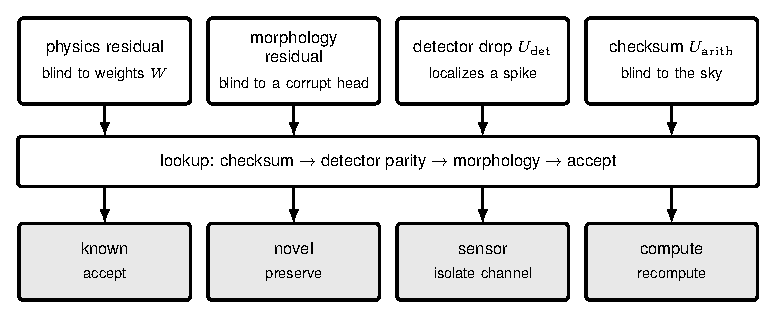
\includegraphics[width=0.92\textwidth]{fig_method.pdf}
\caption{ARIA residuals and lookup. Each residual is forbidden from seeing at least one cause. The decision is a table, not a fused classifier.}
\label{fig:method}
\end{figure}

Two optional bits are evaluated later and are not part of~\eqref{eq:lookup}. The first is a short-window spike score: the worst detector's two-bin excess over the median of the other detectors, scaled by the square root of that median. It fires when the score exceeds the 96th percentile of clean known cubes, times $1.25$, and dropping that detector reduces the score by the same drop fraction $0.28$. The second is a two-fault label. If $U_{\mathrm{arith}}$ and the sensor bit are both true, the lookup in~\eqref{eq:lookup} still says compute, because the checksum is first. An alternative rule returns ``multiple'' instead of choosing. That rule does not change any single-fault row.

\subsection{Simulator}

Each trial draws a sky position, a family template (fast-rise exponential-decay for GRB and SGR, a wide Gaussian for a solar flare, a millisecond TGF), Poisson NaI-like counts with a cosine response, and optional faults. Sensor faults add a soft spike on a dim detector. Compute faults flip one IEEE-754 bit of a linear-head weight, mild bits 18--23 or critical bits 28--30, and revert afterward~\cite{pytorchfi2020,li2017,ieee754}. The head is a standardized linear classifier on $\phi(X)$, not the convolutional-recurrent network of John and colleagues~\cite{john2025}. Inference is emulated in binary32. Binary64 and binary16 are sensitivity checks. The physics residual never needs the head.

Class counts in Table~\ref{tab:cat} are from the HEASARC \texttt{fermigtrig} table on 17 September 2026. They justify holding TGF out as a frequent, morphologically distinct family~\cite{roberts2018,briggs2013}, and they record that the charged-particle triggers are not used as light curves. The simulator's single-detector spike only loosely mimics those particle events.

\begin{table}[t]
\caption{Public Fermi-GBM trigger types used as class priors (HEASARC \texttt{fermigtrig}, 17 September 2026).}
\label{tab:cat}
\centering
\begin{tabular}{lrl}
\toprule
Type & Count & Role in this paper \\
\midrule
GRB & \CatalogGRB{} & known class \\
SFLARE & \CatalogSflare{} & known class \\
SGR & \CatalogSGR{} & known class \\
TGF & \CatalogTGF{} & held-out novel class \\
LOCLPAR+DISTPAR & 2167 & particle events, not used as data \\
All triggers & \CatalogTotal{} & \\
\bottomrule
\end{tabular}
\end{table}

\subsection{Baselines}

Energy and maximum-softmax rejection follow the open-set-score-as-fault-detector idea~\cite{gavarini2022,hendrycks2017,liu2020}: an unusual score is an undifferentiated anomaly. The range check follows ProGIP's magnitude idea~\cite{progip2025}: an extreme logit magnitude is compute, a leftover unusual score is novel, and anything else is known. The range check has no sensor symbol.

\subsection{Protocols}

The headline simulator uses training seeds $\{7,19,31,43,61\}$, evaluation seed $123$, and $36$ trials in each cell of the three known classes clean, TGF clean, sensor on GRB and on SGR, and mild and critical compute on GRB. That is $288$ four-way trials per seed. Thresholds use a disjoint clean calibration stream. Ablations reuse the same signatures with subsets of~\eqref{eq:lookup}. Compound trials inject a spike and a bit-flip together ($n=80$ per training seed in the signature study; the headline count uses one trained head and $n=80$).

The headline real-data protocol trains on all GRB, SGR, and solar-flare cubes in a slice and scores known-clean rows on those same cubes. TGF is never in the training set. Sensor spikes and critical bit-flips are injected on the first $40$ known cubes in file order, which is why the run has \RealTrials{} trials. That prefix contains every GRB in the slice, $15$ SGRs, and no solar flare. The same pipeline is therefore also reported with an injection on every known cube. Mild flips (bits 18--23) are reported on the same $40$ cubes. Five-fold cross-validation, repeated five times, trains on four folds and scores the held-out fold, including its injections. A stratified half-split cuts each family in two, trains on one half, and scores the other, in both directions. The two halves share no trigger name. They are still two halves of one committed slice of \RealCubes{} triggers, not a second catalog draw.

\section{Results}
\label{sec:results}

\subsection{Four-way attribution}

Table~\ref{tab:main} reports mean and standard deviation over the five seeds. ARIA reaches $\AriaAcc\%$ four-way accuracy. The range check reaches $\RangeAcc\%$. Held-out TGF is isolated as novel in $\NovelIso\%$ of trials and is named compute in $\NovelAsCompute\%$. Compute isolation is $\ComputeIso\%$. Sensor isolation is $\SensorIso\%$: the physics residual misses some dim-detector spikes, and those trials fall through to known. That miss rate is reported rather than retuned until the number is round.

\begin{table}[t]
\caption{Four-way accuracy and per-cause isolation in the simulator (percent). Mean $\pm$ standard deviation over five training seeds.}
\label{tab:main}
\centering
\begin{tabular}{lcc}
\toprule
Metric & ARIA & Range check \\
\midrule
Four-way accuracy & $\AriaAcc$ & $\RangeAcc$ \\
Novel $\to$ novel & $\NovelIso$ & -- \\
Novel $\to$ compute & $\NovelAsCompute$ & -- \\
Compute $\to$ compute & $\ComputeIso$ & -- \\
Sensor $\to$ sensor & $\SensorIso$ & 0 (no sensor symbol) \\
\bottomrule
\end{tabular}
\end{table}

Table~\ref{tab:seeds} and Fig.~\ref{fig:seeds} give the per-seed values. ARIA moves by at most $1.4$ points across seeds. The range check moves from $35.8\%$ to $50.7\%$.

\begin{table}[t]
\caption{Per-seed simulator results (percent), evaluation seed 123. ARIA and Range are four-way accuracy. Nov., Comp., and Sens.\ are ARIA isolation of novel, compute, and sensor trials. E/MSP is the share of compute trials flagged by energy or maximum-softmax rejection.}
\label{tab:seeds}
\centering
\small
\begin{tabular}{ccccccc}
\toprule
Seed & ARIA & Range & Nov. & Comp. & Sens. & E/MSP \\
\midrule
7 & 90.6 & 49.7 & 97.2 & 100.0 & 77.8 & 15.3 \\
19 & 90.6 & 35.8 & 100.0 & 100.0 & 77.8 & 20.8 \\
31 & 89.2 & 40.3 & 91.7 & 100.0 & 76.4 & 25.0 \\
43 & 89.6 & 38.9 & 94.4 & 100.0 & 77.8 & 15.3 \\
61 & 89.9 & 50.7 & 91.7 & 100.0 & 77.8 & 8.3 \\
\bottomrule
\end{tabular}
\end{table}


\begin{figure}[t]
\centering
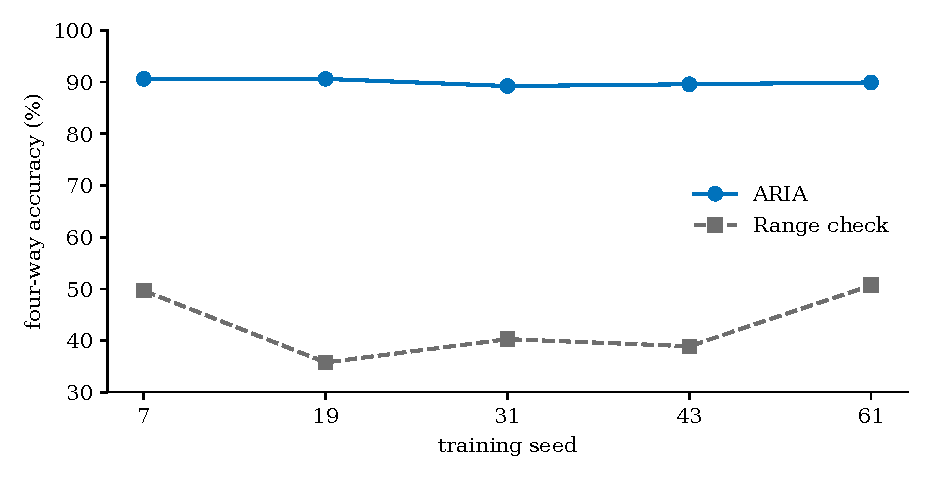
\includegraphics[width=0.78\textwidth]{fig_seeds.pdf}
\caption{Four-way accuracy by training seed, from Table~\ref{tab:seeds}. ARIA stays near $90\%$ on every seed. The range check varies by about $15$ points.}
\label{fig:seeds}
\end{figure}

A representative confusion matrix, training seed $7$, is Table~\ref{tab:conf} and Fig.~\ref{fig:conf}. Energy and maximum-softmax rejection flag $100\%$ of novel trials as an anomaly and between $8.3\%$ and $25.0\%$ of compute trials depending on the seed (mean $16.9\%$). The same rejector fires on discovery and on some bit-flips, and it cannot name either.

\begin{table}[t]
\caption{ARIA confusion counts for training seed 7 in the simulator (36 trials in the novel row and in each compute half; 108 known-clean trials; 72 sensor trials).}
\label{tab:conf}
\centering
\small
\begin{tabular}{lcccc}
\toprule
True $\backslash$ predicted & known & novel & sensor & compute \\
\midrule
known & 98 & 0 & 10 & 0 \\
novel & 0 & 35 & 0 & 1 \\
sensor & 15 & 1 & 56 & 0 \\
compute & 0 & 0 & 0 & 72 \\
\bottomrule
\end{tabular}
\end{table}


\begin{figure}[t]
\centering
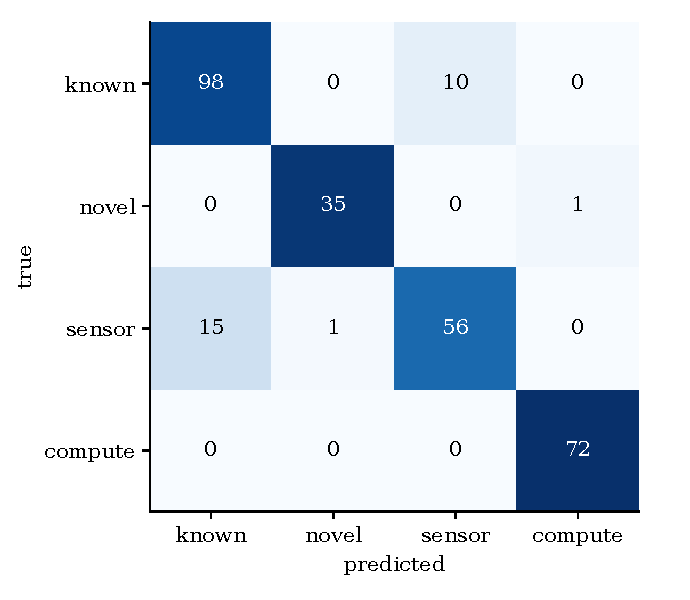
\includegraphics[width=0.62\textwidth]{fig_confusion.pdf}
\caption{ARIA confusion counts for training seed $7$, the same counts as Table~\ref{tab:conf}. Shading is the row-normalized rate. The main errors are missed sensor spikes, clean events called sensor, and one held-out TGF called compute.}
\label{fig:conf}
\end{figure}

\subsection{Checksum calibration, precision, and the rounding bound}
\label{sec:bounded}

The checksum threshold is set on clean residuals only. With that rule, compute isolation is $100\%$ in binary32 and binary64, but the held-out TGF is named compute in $\NovelAsCompute\%$ of binary32 trials. A TGF lies far from the calibration range, so its rounding noise can exceed a threshold calibrated on known classes. The checksum is blind to the sky in exact arithmetic, and not exactly so in finite precision.

Table~\ref{tab:modes} compares the calibrated threshold with the bound~\eqref{eq:bound} on the same trials. At binary32 the bounded rule names no TGF a compute fault (\BndNovCompThirtyTwo\%), keeps compute isolation at \BndCompThirtyTwo\%, including mild flips, and reaches \BndAccThirtyTwo\% four-way accuracy against \CalAccThirtyTwo\% for the calibrated rule. Figure~\ref{fig:checkscatter} shows why. In the calibrated panel a share of the TGF trials sits above the dotted threshold. In the bounded panel every fault-free trial, TGF included, is below $1$, and every flip in the protocol is above it. Figure~\ref{fig:checkroc} shows that at binary32 both statistics rank every compute trial above every TGF trial, so the false-compute rate of the calibrated rule comes from where its threshold sits, not from the residual being unable to rank the two causes.

The guarantee has a price at binary16. Compute isolation falls to \BndCompSixteen\% for the bound against \CalCompSixteen\% for the calibrated rule, and mild flips are caught in \BndMildSixteen\% of trials against \CalMildSixteen\% (Fig.~\ref{fig:checkprec}). Figure~\ref{fig:checkbits} breaks detection down by the flipped bit. The lowest mantissa bits are missed by every variant, because they move a weight by less than the arithmetic's own noise. At binary32 the calibrated rule reaches high detection from bit~8 and the bounded rule from bit~12. The bounded rule trades sensitivity for a guarantee of no false alarm on fault-free inputs.

As a soundness check, $\BoundInputs$ fault-free random inputs per precision were drawn up to $\BoundMaxSigma$ standard deviations from the training mean. The largest ratio of residual to bound was $\BoundWorstRatio$, and none exceeded $1$. This checks the bound on this head. It is not a proof for other heads, and a fault in the stored vectors themselves is outside the model.

% Auto-generated by make_check_figures.py. Do not edit by hand.
\begin{table*}[!t]
\caption{Calibrated and rounding-error-bounded checksum in the simulator (percent, mean $\pm$ standard deviation over five seeds).}
\label{tab:modes}
\centering
\small
\setlength{\tabcolsep}{4pt}
\resizebox{\textwidth}{!}{%
\begin{tabular}{llccccc}
\toprule
Checksum & Prec. & Acc. & Nov.$\to$comp. & Comp.\ (all) & Comp.\ (mild) & Known$\to$comp. \\
\midrule
calibrated & fp64 & 90.1 $\pm$ 0.5 & 3.9 $\pm$ 4.2 & 100.0 $\pm$ 0.0 & 100.0 $\pm$ 0.0 & 0.4 $\pm$ 0.5 \\
calibrated & fp32 & 90.0 $\pm$ 0.6 & 5.0 $\pm$ 3.2 & 100.0 $\pm$ 0.0 & 100.0 $\pm$ 0.0 & 0.4 $\pm$ 0.5 \\
calibrated & fp16 & 86.3 $\pm$ 1.2 & 4.4 $\pm$ 6.2 & 84.2 $\pm$ 5.0 & 76.1 $\pm$ 6.0 & 0.2 $\pm$ 0.4 \\
\midrule
bounded & fp64 & 90.8 $\pm$ 0.2 & 0.0 $\pm$ 0.0 & 100.0 $\pm$ 0.0 & 100.0 $\pm$ 0.0 & 0.0 $\pm$ 0.0 \\
bounded & fp32 & 90.8 $\pm$ 0.2 & 0.0 $\pm$ 0.0 & 100.0 $\pm$ 0.0 & 100.0 $\pm$ 0.0 & 0.0 $\pm$ 0.0 \\
bounded & fp16 & 77.4 $\pm$ 0.3 & 0.0 $\pm$ 0.0 & 46.1 $\pm$ 1.0 & 15.6 $\pm$ 1.4 & 0.0 $\pm$ 0.0 \\
\bottomrule
\end{tabular}}
\end{table*}

\begin{table}[!t]
\caption{Calibrated and bounded checksum on real CTIME (\%, mean over five training seeds; the across-seed spread is $0.0$ in every cell, as explained in Section~\ref{sec:real}). Triggers per class; compute faults are critical flips only. Nov.$\to$comp.: held-out TGF named compute.}
\label{tab:realmodes}
\centering
\small
\setlength{\tabcolsep}{3pt}
\begin{tabular}{llccccc}
\toprule
Checksum & Prec. & n/cl. & Acc. & Comp. & Sens. & Nov.$\to$comp. \\
\midrule
calibrated & fp32 & 8 & 76.3 & 100.0 & 58.3 & 0.0 \\
calibrated & fp32 & 12 & 76.7 & 100.0 & 61.1 & 8.3 \\
calibrated & fp32 & 25 & 74.4 & 100.0 & 60.0 & 0.0 \\
calibrated & fp16 & 8 & 73.8 & 100.0 & 54.2 & 12.5 \\
calibrated & fp16 & 12 & 77.5 & 100.0 & 63.9 & 0.0 \\
calibrated & fp16 & 25 & 74.4 & 100.0 & 60.0 & 0.0 \\
\midrule
bounded & fp32 & 8 & 80.0 & 100.0 & 70.8 & 0.0 \\
bounded & fp32 & 12 & 77.5 & 100.0 & 63.9 & 0.0 \\
bounded & fp32 & 25 & 74.4 & 100.0 & 60.0 & 0.0 \\
bounded & fp16 & 8 & 73.8 & 79.2 & 70.8 & 0.0 \\
bounded & fp16 & 12 & 75.0 & 91.7 & 63.9 & 0.0 \\
bounded & fp16 & 25 & 73.3 & 95.0 & 60.0 & 0.0 \\
\bottomrule
\end{tabular}
\end{table}


\begin{figure*}[t]
\centering
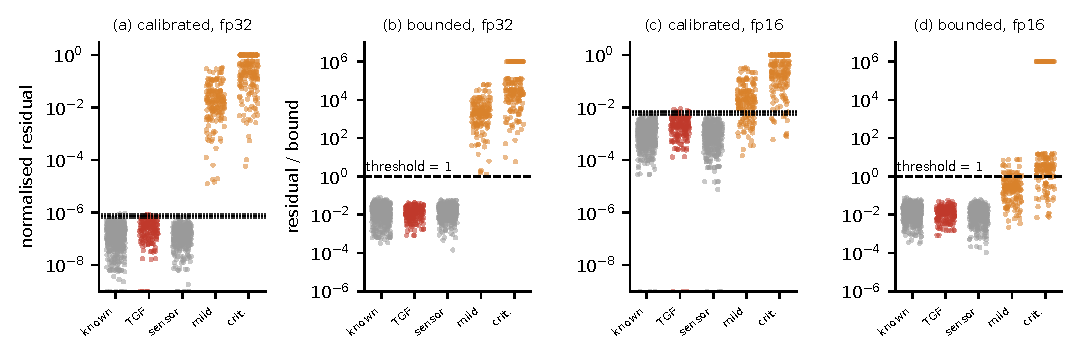
\includegraphics[width=\textwidth]{fig_check_scatter.pdf}
\caption{Checksum statistic of every simulator trial, five seeds pooled, by true cause. Panels (a) and (c) are the calibrated normalized residual, with per-seed thresholds dotted. Panels (b) and (d) divide the residual by the bound~\eqref{eq:bound}, with the decision threshold at $1$ dashed. Panels (a) and (b) are binary32. Panels (c) and (d) are binary16. Compute trials are orange. The held-out TGF is red. Counts are in Table~\ref{tab:modes}.}
\label{fig:checkscatter}
\end{figure*}

\begin{figure}[t]
\centering
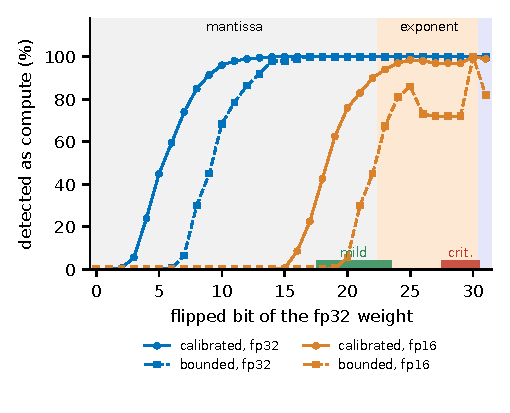
\includegraphics[width=0.72\textwidth]{fig_check_bits.pdf}
\caption{Share of single bit-flips detected as compute, against the flipped bit of the binary32 weight (200 flips per bit, five seeds, fault-free known-class events). Circles are the calibrated rule. Squares are the bounded rule. The shaded bands mark mantissa, exponent, and sign. The bars at the bottom mark the mild range (bits 18--23) and the critical range (bits 28--30) used in the main protocol.}
\label{fig:checkbits}
\end{figure}

\begin{figure}[t]
\centering
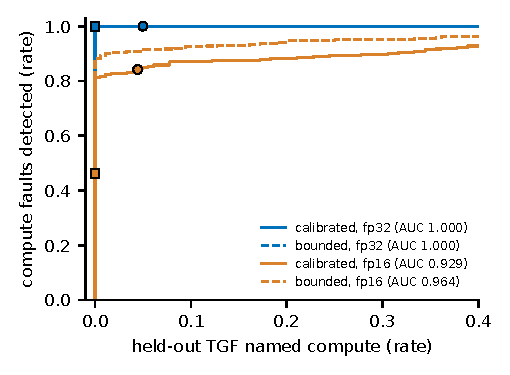
\includegraphics[width=0.72\textwidth]{fig_check_roc.pdf}
\caption{Compute faults detected, against held-out TGFs named compute, as the checksum threshold is swept (five seeds pooled). The marker is the operating point actually used: the per-seed calibrated threshold, or the bound threshold $1$.}
\label{fig:checkroc}
\end{figure}

\begin{figure}[t]
\centering
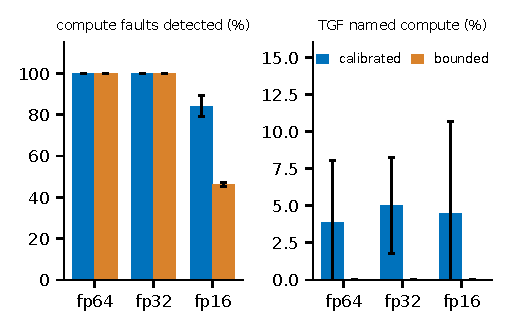
\includegraphics[width=0.72\textwidth]{fig_check_prec.pdf}
\caption{Calibrated and bounded checksums at three inference precisions (mean $\pm$ standard deviation over five seeds; values in Table~\ref{tab:modes}). The bounded rule never names a TGF compute in the simulator. It loses compute sensitivity at binary16.}
\label{fig:checkprec}
\end{figure}

On real CTIME the same comparison is Table~\ref{tab:realmodes}. At binary32 the bounded rule keeps compute isolation at $100\%$ and names no TGF compute at any slice size, while the calibrated rule names $\RealCalNovCompTwelve\%$ of TGFs as compute at $12$ triggers per class. Sensor isolation at eight triggers per class is $\RealBndSensEight\%$ for the bound against $\RealCalSensEight\%$ for the calibrated rule, because some spiked cubes trip the calibrated checksum and are therefore labeled compute before the sensor bit is read. At the $25$-cube slice the two rules agree. Novel isolation stays at $0\%$ in every row. That limit comes from the CTIME bins, not from the checksum.

\subsection{Ablations}

Table~\ref{tab:abl} and Fig.~\ref{fig:abl} remove signature bits. A checksum alone cannot name novelty or sensors ($\AblChecksum\%$). Physics alone names some sensors and defaults everyone else to known ($\AblPhysics\%$). Morphology alone is an open-set detector ($\AblMorph\%$). Removing only the checksum drops accuracy to $\AblNoChecksum\%$, because compute trials fall into known or novel. Full ARIA is $\AblFull\%$. Each residual covers a cause the others cannot see.

\begin{table}[t]
\caption{Ablation of the lookup. Four-way accuracy, percent, mean $\pm$ standard deviation over five seeds.}
\label{tab:abl}
\centering
\begin{tabular}{lc}
\toprule
Lookup & Accuracy \\
\midrule
Full ARIA, equation~\eqref{eq:lookup} & $\AblFull$ \\
Checksum only & $\AblChecksum$ \\
Physics only & $\AblPhysics$ \\
Morphology only & $\AblMorph$ \\
No checksum & $\AblNoChecksum$ \\
\bottomrule
\end{tabular}
\end{table}

\begin{figure}[t]
\centering
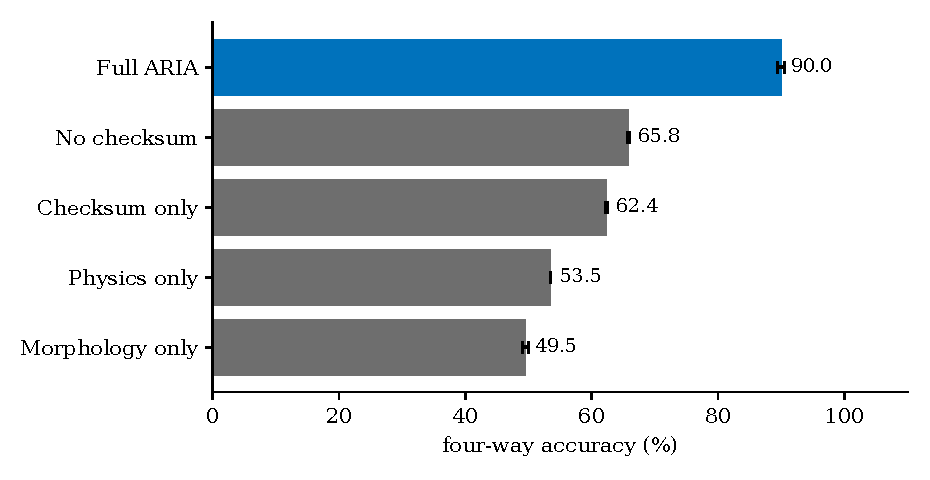
\includegraphics[width=0.78\textwidth]{fig_ablation.pdf}
\caption{Ablation of the lookup. Values are in Table~\ref{tab:abl}. Every residual alone is far below the full dictionary.}
\label{fig:abl}
\end{figure}

\subsection{Summary against the baselines}

Table~\ref{tab:summary} puts ARIA next to the two baselines on the simulator and on real CTIME. Only ARIA names a cause for novelty, compute faults, and sensors. On novelty it pays a small false-compute rate in the simulator under the calibrated checksum. Energy and maximum-softmax rejection never name a cause.

\begin{table*}[t]
\caption{Summary of the headline results (percent, mean $\pm$ standard deviation over five training seeds). A dash means the method does not produce that output. Flag novel and flag compute are the share of those trials that energy or maximum-softmax rejection marks as an undifferentiated anomaly.}
\label{tab:summary}
\centering
\footnotesize
\setlength{\tabcolsep}{3pt}
\resizebox{\textwidth}{!}{%
\begin{tabular}{llccccccc}
\toprule
Setting & Method & Four-way & Novel & Compute & Sensor & Nov.$\to$comp. & Flag novel & Flag compute \\
\midrule
\multirow{3}{*}{Simulator}
& ARIA & $\AriaAcc$ & $\NovelIso$ & $\ComputeIso$ & $\SensorIso$ & $\NovelAsCompute$ & -- & -- \\
& Range check & $\RangeAcc$ & -- & -- & 0 & -- & -- & -- \\
& Energy / MSP & -- & -- & -- & -- & -- & $100.0\pm0.0$ & $16.9\pm5.7$ \\
\midrule
\multirow{3}{*}{Real CTIME}
& ARIA & $\RealAriaAccPM$ & $\RealNovelIsoPM$ & $\RealComputeIsoPM$ & $\RealSensorIsoPM$ & $\RealNovelAsComputePM$ & -- & -- \\
& Range check & $\RealRangeAccPM$ & -- & -- & 0 & -- & -- & -- \\
& Energy / MSP & -- & -- & -- & -- & -- & $\RealEnergyNovelPM$ & $\RealEnergyComputePM$ \\
\bottomrule
\end{tabular}}
\end{table*}

\subsection{Compound faults}

When a spike and a bit-flip occur together, $U_{\mathrm{arith}}$ still fires, so the headline lookup names compute on $\CompoundCompute\%$ of $80$ compound trials (Table~\ref{tab:compound}). Across five training seeds, both the checksum bit and the sensor bit are true on $\BothSig\%$ of compound trials, and the checksum alone is true on $\ArithOnly\%$ (Fig.~\ref{fig:compound}). The physics bit never fires by itself. The optional two-fault rule therefore returns ``multiple'' on $\MultiRate\%$ of these trials and still returns compute on the rest, where the spike left no physics signature. The dictionary can refuse a single label when both residuals fire. It cannot recover a sensor fault that the physics residual missed. Two causes remain unisolable as a pair of named faults.

\begin{table}[t]
\caption{Headline lookup on 80 compound sensor-plus-compute trials from one trained head. The five-seed signature split is in Fig.~\ref{fig:compound}.}
\label{tab:compound}
\centering
\begin{tabular}{lcccc}
\toprule
 & known & novel & sensor & compute \\
\midrule
Trials named & 0 & 0 & 0 & 80 \\
\bottomrule
\end{tabular}
\end{table}

\begin{figure}[t]
\centering
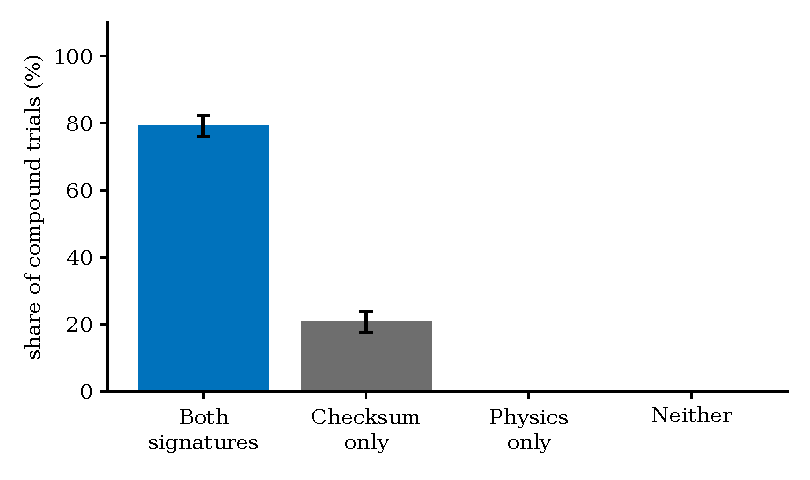
\includegraphics[width=0.72\textwidth]{fig_compound.pdf}
\caption{Which residual bits fire on compound trials (mean $\pm$ standard deviation over five training seeds, 80 trials each). ``Both signatures'' is the share the optional rule labels multiple. The headline lookup labels every one of these trials compute.}
\label{fig:compound}
\end{figure}

\section{Public CTIME measurements}
\label{sec:real}

\subsection{Headline slice}

The download keeps \RealPerClass{} triggers of each of GRB, SGR, solar flare, and TGF, binned to $8\times 64$ light cubes (\RealCubes{} cubes). CTIME bins are coarse, nominally $64$\,ms and $256$\,ms in the background regime. A TGF is sub-millisecond~\cite{briggs2013,roberts2018}. The linear head is trained on all known-class cubes in the slice. Known-clean evaluation reuses those cubes, so four-way accuracy is optimistic on the known-clean rows. TGF is held out entirely. Real-data compute trials use critical flips only in the headline row. The run uses the same five training seeds and evaluation seed $\RealEvalSeed$, with \RealTrials{} trials per seed.

Table~\ref{tab:real} and Fig.~\ref{fig:simreal} compare that run with the simulator. Compute isolation on critical flips is $\RealComputeIso\%$. Held-out TGF is named compute in $\RealNovelAsCompute\%$ of trials at this slice size. Four-way accuracy is $\RealAriaAcc\%$ and sensor isolation is $\RealSensorIso\%$. Novel isolation is $\RealNovelIso\%$. On these bins a TGF is not separable from a short GRB, so held-out TGFs fall through to known. Table~\ref{tab:realconf} shows the calls at training seed $7$: all $25$ TGF cubes are called known, and $29$ of $40$ sensor injections are caught. This is a negative result about the discovery symbol, not a tuning failure. Section~\ref{sec:morph} shows that a lower morphology threshold does not fix it.

\begin{table}[t]
\caption{Public GBM CTIME, \RealPerClass{} triggers per class, software fault injection (percent). Mean $\pm$ standard deviation over \RealSeeds{} training seeds at evaluation seed $\RealEvalSeed$. The simulator column is Table~\ref{tab:main}.}
\label{tab:real}
\centering
\begin{tabular}{lcc}
\toprule
Metric & Real CTIME & Simulator \\
\midrule
Four-way accuracy & $\RealAriaAccPM$ & $\AriaAcc$ \\
Range-check accuracy & $\RealRangeAccPM$ & $\RangeAcc$ \\
Novel $\to$ novel & $\RealNovelIsoPM$ & $\NovelIso$ \\
Novel $\to$ compute & $\RealNovelAsComputePM$ & $\NovelAsCompute$ \\
Compute $\to$ compute & $\RealComputeIsoPM$ & $\ComputeIso$ \\
Sensor $\to$ sensor & $\RealSensorIsoPM$ & $\SensorIso$ \\
\bottomrule
\end{tabular}
\end{table}

\begin{figure}[t]
\centering
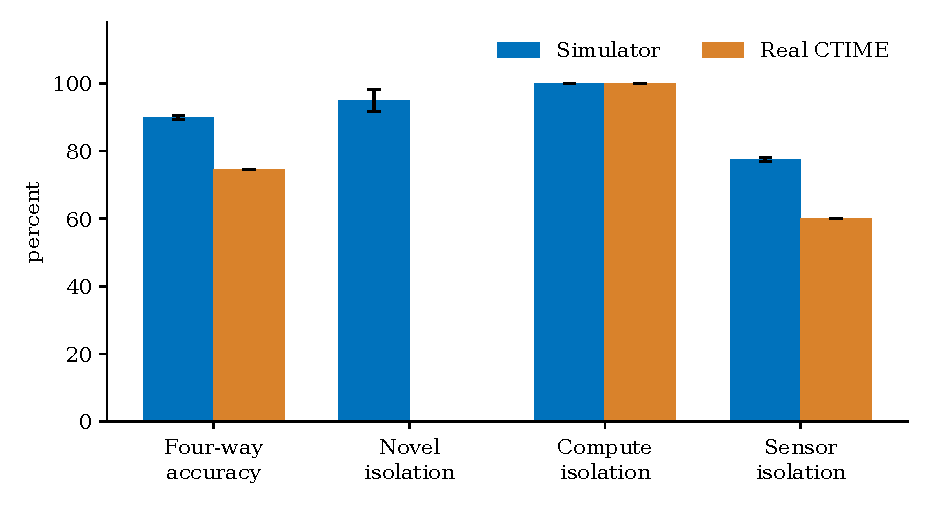
\includegraphics[width=0.78\textwidth]{fig_sim_vs_real.pdf}
\caption{ARIA on the simulator and on real CTIME, from Table~\ref{tab:real}. Compute isolation is high in both settings. The real compute trials are critical flips only. Sensor isolation and four-way accuracy drop. Novel isolation is zero on CTIME.}
\label{fig:simreal}
\end{figure}

\begin{table}[t]
\caption{ARIA calls on the public CTIME slice at training seed 7 and evaluation seed 123, using the published injection budget (the first 40 known cubes). All 25 held-out TGF cubes are called known.}
\label{tab:realconf}
\centering
\small
\begin{tabular}{lcccc}
\toprule
True $\backslash$ predicted & known & novel & sensor & compute \\
\midrule
known & 70 & 2 & 2 & 1 \\
novel & 25 & 0 & 0 & 0 \\
sensor & 16 & 0 & 24 & 0 \\
compute & 0 & 0 & 0 & 40 \\
\bottomrule
\end{tabular}
\end{table}


The across-seed spread on this slice is zero for every headline metric. Clean-only calibration no longer depends on randomly drawn injected faults, and the same cubes train every seed. The spread says nothing about which triggers were drawn. Slice size, cross-validation, and the half-split are the checks on that axis.

\subsection{Slice size}

Figure~\ref{fig:trend} and Table~\ref{tab:trend} repeat the calibrated binary32 pipeline at three slice sizes. The smaller slices are prefixes of the $25$-cube families. Four-way accuracy is $76.3\%$, $76.7\%$, and $74.4\%$. It is not monotone. Compute isolation is $100\%$ at every size. Novel isolation is $0\%$ at every size. The held-out TGF is named compute in $0\%$, $8.3\%$, and $0\%$ of trials, so the false-compute rate on novelty is small, not constant, and not a structural zero.

\begin{figure}[t]
\centering
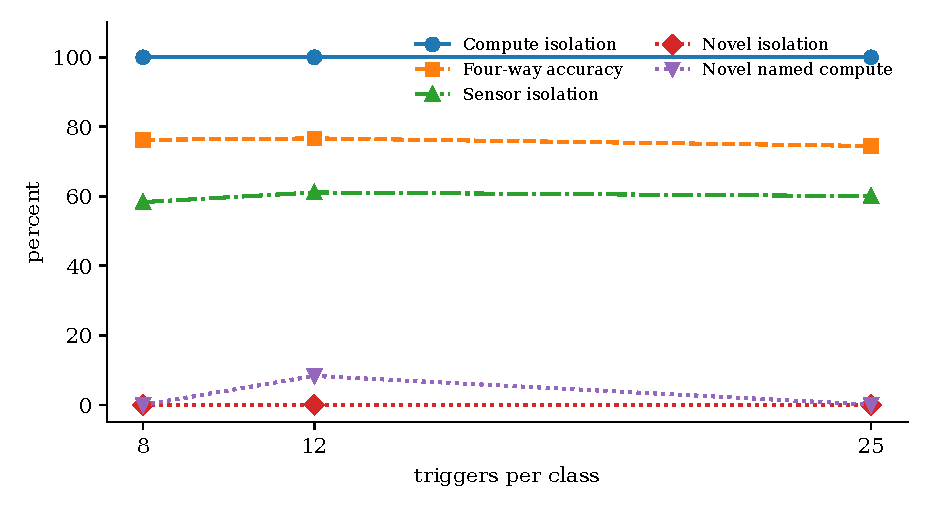
\includegraphics[width=0.78\textwidth]{fig_trend.pdf}
\caption{Real CTIME metrics against slice size, calibrated binary32, from Table~\ref{tab:trend}. Compute isolation stays at $100\%$. Novel isolation stays at $0\%$. The false-compute rate on TGF is not zero at every size.}
\label{fig:trend}
\end{figure}

\begin{table*}[t]
\caption{Calibrated fp32 ARIA on public CTIME as the slice grows (percent, mean over five training seeds). The 8- and 12-cube rows are prefixes of the 25-cube slice.}
\label{tab:trend}
\centering
\small
\begin{tabular}{cccccc}
\toprule
Per class & Acc. & Compute & Sensor & Novel$\to$comp. & Novel \\
\midrule
8 & 76.3 & 100.0 & 58.3 & 0.0 & 0.0 \\
12 & 76.7 & 100.0 & 61.1 & 8.3 & 0.0 \\
25 & 74.4 & 100.0 & 60.0 & 0.0 & 0.0 \\
\bottomrule
\end{tabular}
\end{table*}


\subsection{Why the novel symbol is empty}
\label{sec:morph}

Figure~\ref{fig:morph} and Table~\ref{tab:morph} plot the morphology residual on the clean cubes. The mean distance of TGF to the nearest known centroid is smaller than the mean distance of GRB. No TGF exceeds the shipped threshold. Four solar flares do, which is why a known class, not the held-out class, supplies the morphology false alarms. In the duration--width plane the four families overlap. TGF does not occupy a region the three trained classes leave empty, once the light curve has been averaged into CTIME bins.

\begin{table}[t]
\caption{Morphology distance to the nearest known-class centroid on clean public CTIME cubes (training seed 7). The shipped threshold is 3.98. TGF is closer to the known centroids than GRB is. Above: cubes whose distance exceeds that threshold.}
\label{tab:morph}
\centering
\small
\begin{tabular}{lrrrrr}
\toprule
Family & $n$ & Mean & Min & Max & Above \\
\midrule
GRB & 25 & 1.18 & 0.48 & 2.87 & 0 \\
SGR & 25 & 1.36 & 0.39 & 3.18 & 0 \\
SFLARE & 25 & 2.65 & 0.76 & 9.59 & 4 \\
TGF & 25 & 1.08 & 0.57 & 2.47 & 0 \\
\bottomrule
\end{tabular}
\end{table}


\begin{figure}[t]
\centering
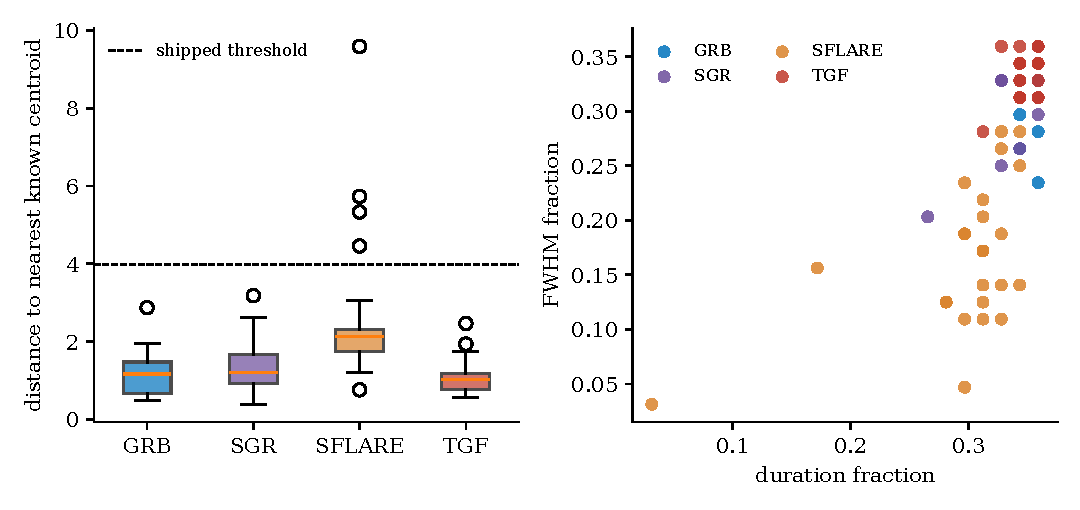
\includegraphics[width=0.92\textwidth]{fig_morph.pdf}
\caption{Left: morphology distance of each clean CTIME cube to the nearest known-class centroid. The dashed line is the shipped threshold. Right: duration fraction against full width at half maximum for the same cubes. TGF sits inside the GRB cloud.}
\label{fig:morph}
\end{figure}

Table~\ref{tab:sweep} and Fig.~\ref{fig:sweep} lower and raise that threshold. The shipped margin is $1.25$ on the clean 95th percentile. At margin $0.5$, novel isolation rises only to $12\%$, while $41.3\%$ of known triggers are called novel and four-way accuracy falls to $60\%$. There is no operating point on this slice at which TGF is recovered and known bursts are still accepted. The discovery symbol needs finer time bins. It does not need a lower threshold.

\begin{table}[t]
\caption{Morphology-threshold sweep on the public CTIME slice (training seed 7, published injection budget). The margin multiplies the 95th percentile of clean known-class morphology distances. The shipped rule uses margin 1.25. Lowering it does not recover TGF as novel without calling a large share of known triggers novel.}
\label{tab:sweep}
\centering
\small
\begin{tabular}{ccccc}
\toprule
Margin & Acc. & Novel & Known$\to$novel & Novel$\to$known \\
\midrule
0.5 & 60.0 & 12.0 & 41.3 & 88.0 \\
0.75 & 72.2 & 4.0 & 9.3 & 96.0 \\
1 & 74.4 & 0.0 & 2.7 & 100.0 \\
1.25 & 74.4 & 0.0 & 2.7 & 100.0 \\
1.5 & 75.0 & 0.0 & 1.3 & 100.0 \\
2 & 75.6 & 0.0 & 0.0 & 100.0 \\
3 & 75.6 & 0.0 & 0.0 & 100.0 \\
4 & 75.6 & 0.0 & 0.0 & 100.0 \\
\bottomrule
\end{tabular}
\end{table}


\begin{figure}[t]
\centering
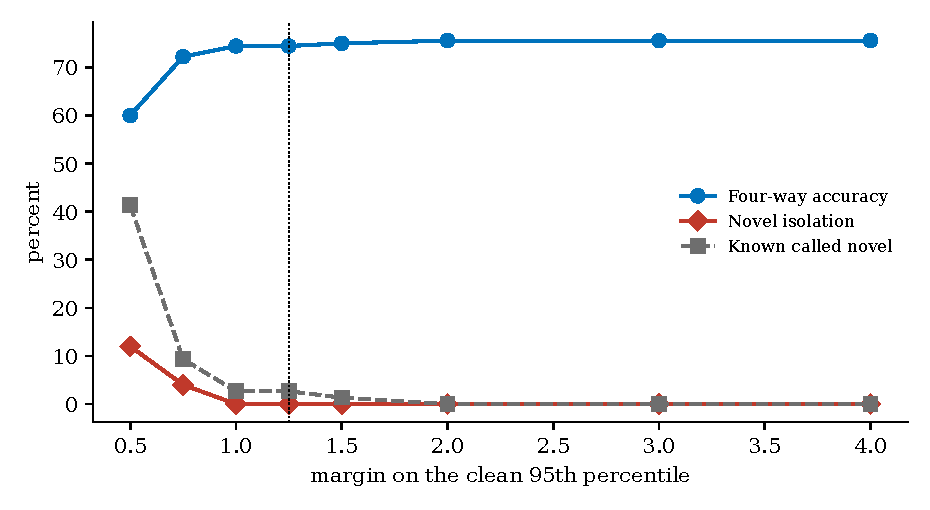
\includegraphics[width=0.78\textwidth]{fig_sweep.pdf}
\caption{Threshold sweep from Table~\ref{tab:sweep}. The dotted line is the shipped margin. Novel isolation stays near zero until known triggers are being rejected in large numbers.}
\label{fig:sweep}
\end{figure}

\section{Checks that were not in the headline table}
\label{sec:extra}

\subsection{Out-of-sample cubes, and the injection budget}

The headline real-data accuracy trains and scores known classes on the same cubes, and it injects faults only into the first $40$ known cubes. Table~\ref{tab:family} shows what that budget is. Every GRB is injected, $15$ of $25$ SGRs are injected, and no solar flare is injected. When every known cube is injected, sensor isolation rises from $\RealSensorIso\%$ to $\AllSens\%$ and four-way accuracy from $\RealAriaAcc\%$ to $\AllAcc\%$. GRB spikes are caught $56\%$ of the time. Solar-flare spikes are caught $80\%$ of the time, and the SGR rate moves from $66.7\%$ on the $15$ cubes inside the prefix to $72\%$ once all $25$ are included. The $60\%$ figure is the GRB-heavy budget, not a property of every family.

\begin{table}[t]
\caption{Sensor isolation by trigger family on public CTIME (percent, pooled over five training seeds). The count in parentheses is the number of injected cubes of that family. The published budget never injects a spike into a solar flare.}
\label{tab:family}
\centering
\small
\begin{tabular}{lccc}
\toprule
Budget & GRB & SGR & SFLARE \\
\midrule
First 40 known cubes & 56.0 (25) & 66.7 (15) & -- \\
Every known cube & 56.0 (25) & 72.0 (25) & 80.0 (25) \\
\bottomrule
\end{tabular}
\end{table}


Table~\ref{tab:protocols} and Fig.~\ref{fig:protocols} score cubes the head was not trained on. Five-fold cross-validation, repeated five times, gives $\CvAcc\%$ accuracy, $\CvComp\%$ compute isolation, $\CvSens\%$ sensor isolation, and $\CvNovelComp\%$ of TGFs named compute. Novel isolation remains $\CvNovel\%$. The half-split agrees in both directions: accuracy $\SplitABAcc\%$ and $\SplitBAAcc\%$, sensor isolation $\SplitABSens\%$ and $\SplitBASens\%$, compute isolation $100\%$, and no TGF named compute. The in-sample headline is not an outlier relative to these splits of one slice. The seed-to-seed standard deviation of zero on the headline row was the wrong uncertainty. The fold-to-fold sensor spread, $\pm 7.5$ points, is the uncertainty this slice can support. A second catalog draw is reported below, and it moves sensor isolation by much more than the folds do. Mild bit-flips, bits 18--23, are isolated as compute on $\MildComp\%$ of the published injection budget, the same rate as critical flips, under the calibrated binary32 rule. The flips that stay invisible are the low mantissa bits in Fig.~\ref{fig:checkbits}, not this mild band.

\begin{table*}[t]
\caption{Public CTIME outside the headline protocol (percent). Neither split is a new catalog draw.}
\label{tab:protocols}
\centering
\small
\resizebox{\textwidth}{!}{%
\begin{tabular}{lccccc}
\toprule
Protocol & Acc. & Compute & Sensor & Nov.$\to$comp. & Novel \\
\midrule
In-sample, first 40 known cubes & 74.4 $\pm$ 0.0 & 100.0 $\pm$ 0.0 & 60.0 $\pm$ 0.0 & 0.0 $\pm$ 0.0 & 0.0 $\pm$ 0.0 \\
In-sample, every known cube & 78.8 $\pm$ 0.0 & 100.0 $\pm$ 0.0 & 69.3 $\pm$ 0.0 & 0.0 $\pm$ 0.0 & 0.0 $\pm$ 0.0 \\
Mild flips, first 40 known cubes & 74.4 $\pm$ 0.0 & 100.0 $\pm$ 0.0 & 60.0 $\pm$ 0.0 & 0.0 $\pm$ 0.0 & 0.0 $\pm$ 0.0 \\
5$\times$5 cross-validation & 77.2 $\pm$ 2.7 & 100.0 $\pm$ 0.0 & 65.3 $\pm$ 7.5 & 0.0 $\pm$ 0.0 & 0.0 $\pm$ 0.0 \\
Half-split, A$\to$B & 77.7 $\pm$ 0.0 & 100.0 $\pm$ 0.0 & 66.7 $\pm$ 0.0 & 0.0 $\pm$ 0.0 & 0.0 $\pm$ 0.0 \\
Half-split, B$\to$A & 80.0 $\pm$ 0.0 & 100.0 $\pm$ 0.0 & 72.2 $\pm$ 0.0 & 0.0 $\pm$ 0.0 & 0.0 $\pm$ 0.0 \\
\bottomrule
\end{tabular}}
\end{table*}


\begin{figure}[t]
\centering
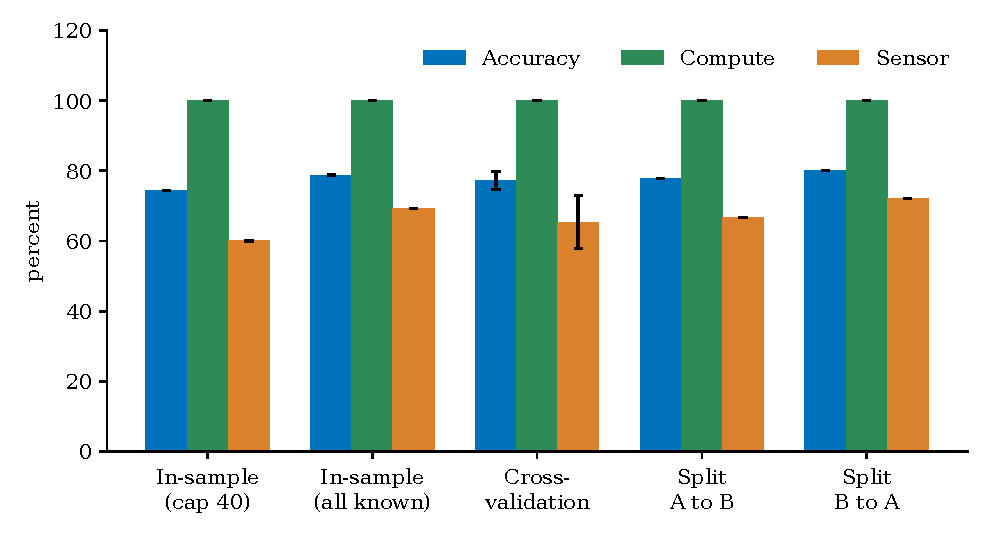
\includegraphics[width=0.86\textwidth]{fig_protocols.pdf}
\caption{Public CTIME under the protocols of Table~\ref{tab:protocols}. Compute isolation stays at $100\%$. Accuracy stays in a band around the headline $74.4\%$. Sensor isolation is the quantity that moves.}
\label{fig:protocols}
\end{figure}

\subsection{Short-window spike score}

The physics residual is a full-curve cosine. A two-bin spike is a small fraction of a $64$-bin inner product, which is a plausible reason sensor isolation is the weak cell. The short-window score in Section~3 was built to test that reason. Its threshold uses clean cubes only.

Table~\ref{tab:spike} and Fig.~\ref{fig:spike} are the result. On the simulator, adding the bit raises sensor isolation from $\SimHeadSens\%$ to $\SimSpikeSens\%$ and four-way accuracy from the headline to $\SimSpikeAcc\%$, while known events called sensor stay near $\SimHeadKnown\%$ and $\SimSpikeKnown\%$. On the published CTIME budget the same bit leaves sensor isolation at $\RealSpikeSens\%$ and accuracy at $\RealSpikeAcc\%$. Novel events called sensor stay at $\RealSpikeNovS\%$. The obvious short-window correction repairs the simulator and does not repair the public cubes. A Poisson matched filter that uses the real NaI response~\cite{perera2025} is still open. It is not what was measured here.

\begin{table*}[t]
\caption{Short-window spike score, thresholded on clean cubes only and OR-ed into the sensor bit (percent). On the simulator the bit raises sensor isolation. On the published CTIME budget it does not.}
\label{tab:spike}
\centering
\small
\resizebox{\textwidth}{!}{%
\begin{tabular}{lcccc}
\toprule
Rule & Acc. & Sensor & Known$\to$sensor & Novel$\to$sensor \\
\midrule
Simulator, headline & 90.0 $\pm$ 0.6 & 77.5 $\pm$ 0.6 & 9.3 $\pm$ 0.0 & 0.0 $\pm$ 0.0 \\
Simulator, spike bit added & 92.2 $\pm$ 0.6 & 86.7 $\pm$ 0.7 & 9.4 $\pm$ 0.4 & 0.0 $\pm$ 0.0 \\
CTIME, headline & 74.4 $\pm$ 0.0 & 60.0 $\pm$ 0.0 & 2.7 $\pm$ 0.0 & 0.0 $\pm$ 0.0 \\
CTIME, spike bit added & 74.4 $\pm$ 0.0 & 60.0 $\pm$ 0.0 & 2.7 $\pm$ 0.0 & 0.0 $\pm$ 0.0 \\
\bottomrule
\end{tabular}}
\end{table*}


\begin{figure}[t]
\centering
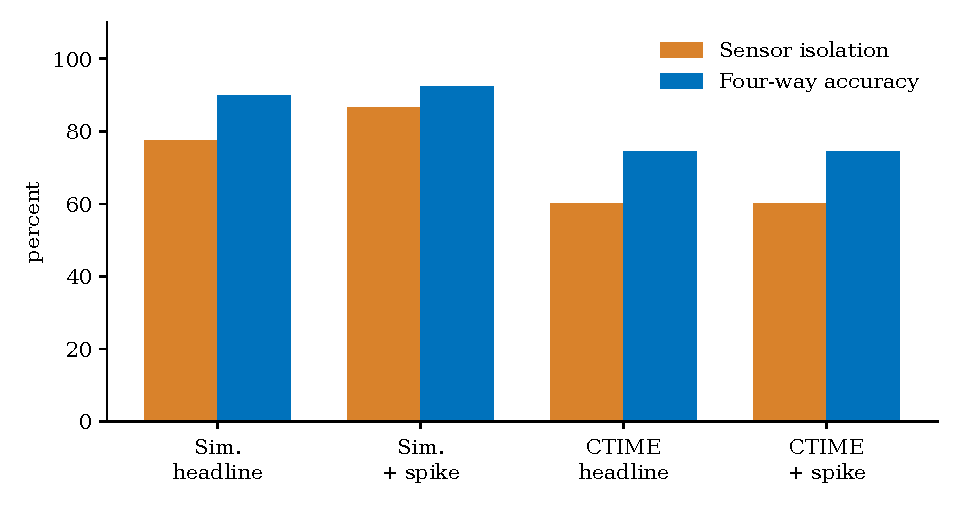
\includegraphics[width=0.78\textwidth]{fig_spike.pdf}
\caption{Sensor isolation and four-way accuracy with and without the short-window spike bit, from Table~\ref{tab:spike}. The bit helps the simulator. It does not move the public CTIME result.}
\label{fig:spike}
\end{figure}

\subsection{A second catalog draw}
\label{sec:draw2}

The half-split reshuffles one download. Table~\ref{tab:draw} is a second download: 25 triggers in each of the four families, no name in common with the published slice, binned by the same CTIME procedure. Training on draw~1 and scoring draw~2 gives 70.6\% four-way accuracy, 100\% compute isolation, 65\% sensor isolation, and no TGF called novel or compute. The other direction gives 62.8\% accuracy and 7.5\% sensor isolation, with compute isolation still 100\% and the novel symbol still empty. Draw~2 scored on itself is already at 25\% sensor isolation.

The mechanism is the clip on the physics threshold. On draw~1 the clean residuals sit low, so the threshold takes its floor, $0.38$. On draw~2 they sit high, so the threshold takes its ceiling, $0.62$. Injected spikes on either draw have a median physics residual near $0.4$. They clear $0.38$ about as often as the headline $60\%$, and they mostly miss $0.62$. Compute isolation and the empty novel symbol are the results that survive a new draw. The sensor rate does not.

Removing the clip, and refitting the same percentile, widens the disagreement. Training on draw~1 and scoring draw~2 then isolates $87.5\%$ of spikes and names $9.3\%$ of clean known cubes a sensor fault. The other direction isolates $5.0\%$. The floor and the ceiling were pulling the two thresholds toward each other. Table~\ref{tab:draw} keeps the clip.

\begin{table*}[t]
\caption{Disjoint CTIME draws (percent). Draw~2 shares no trigger name with the published slice. Seed-to-seed spread is zero.}
\label{tab:draw}
\centering
\small
\begin{tabular}{lccccc}
\toprule
Train $\to$ score & Accuracy & Compute & Sensor & Novel & Novel$\to$compute \\
\midrule
Draw 1 $\to$ draw 1 & 74.4 & 100 & 60.0 & 0 & 0 \\
Draw 1 $\to$ draw 2 & 70.6 & 100 & 65.0 & 0 & 0 \\
Draw 2 $\to$ draw 2 & 67.8 & 100 & 25.0 & 0 & 0 \\
Draw 2 $\to$ draw 1 & 62.8 & 100 & 7.5 & 0 & 0 \\
\bottomrule
\end{tabular}
\end{table*}


\subsection{Millisecond light curves}
\label{sec:tte}

The CTIME novel symbol is empty because a sub-millisecond flash occupies one 64\,ms bin. The same GRB and TGF names were therefore rebinned from time-tagged event files at 1\,ms, on a window from $0.5$\,s before the trigger to $1.5$\,s after. One flash, \texttt{bn260414904}, had no usable eight-detector file, leaving 25 bursts and 24 flashes. Background for each detector is the median of $[-0.5,-0.1)$\,s. The CTIME estimator, which reads only the first and last eight bins, is not applied to the raw 2\,s window.

Distance is Euclidean in the eight morphology features, standardized on the bursts. Each burst is scored against the centroid of the other bursts. The threshold is the 95th percentile of those distances, times the same $1.25$ margin used by the lookup. Flashes are scored against the centroid of every burst. Figure~\ref{fig:tte} shows the result. The threshold is $5.21$. One of 25 bursts lies above it. Twenty-three of 24 flashes lie above it. The flash that does not, \texttt{bn120312139}, has a full width at half maximum of $1.2$\,s in this window, against about $1$\,ms for the flashes that separate and about $2$\,s for a typical burst here. This is a GRB-only centroid, on the download that skipped \texttt{bn260414904}. It is a distance, not a lookup label.

The lookup was then run on a later file from the same window: 25 triggers in each of GRB, SGR, solar flare, and TGF, including \texttt{bn260414904}. Background is the same pre-trigger median. The head trains on the three known classes. No fault is injected. All five seeds agree. The physics threshold sits on the clip ceiling, $0.62$. Median physics residuals are $0.986$ (GRB), $0.974$ (SGR), $1$ (solar flare), and $0.954$ (TGF). That residual clears the ceiling for every burst, every magnetar burst, every flash, and 23 of 25 flares. The morphology threshold is $5.85$. The morphology bit is true for 1 of 25 flashes, 1 of 25 magnetar bursts, 2 of 25 flares, and no burst. Those two flares are the only novel calls, because their physics residual stays under the ceiling. The checksum threshold is $6.31\times 10^{-7}$. The median checksum on flashes is $1.40\times 10^{-7}$, under the threshold, so the compute symbol stays off. Table~\ref{tab:ttelookup} names every flash a sensor fault. The detectors at 1\,ms do not share one smooth profile, and the lookup reads that bit before it reads morphology.

Summing the same photons to 8, 16, and 50\,ms, and switching to the ordinary eight-bin background, leaves the same call. Median physics residuals are $1$ in every family at 8 and 16\,ms, and still $1$ for bursts, magnetar bursts, and flashes at 50\,ms ($0.92$ for flares). At 8\,ms, 24 flashes are sensor and one is compute. At 16 and 50\,ms all 25 flashes are sensor. At 50\,ms, seven flares and two magnetar bursts fall through to known, and one flare is named compute. Wider bins do not hand the novel symbol back. Native CTIME, near 64\,ms, is the case already reported, and there the flashes are called known.

\begin{table}[t]
\caption{Lookup calls on time-tagged photons, with no injected fault. Each count is out of 25. Every training seed returns the same row. The 1\,ms row subtracts a pre-trigger background. The other rows sum that file and use the first and last eight bins.}
\label{tab:ttelookup}
\centering
\small
\begin{tabular}{llrrrr}
\toprule
Bin & Family & Sensor & Known & Novel & Compute \\
\midrule
\multirow{4}{*}{1\,ms}
 & GRB & 25 & 0 & 0 & 0 \\
 & SGR & 25 & 0 & 0 & 0 \\
 & Solar flare & 23 & 0 & 2 & 0 \\
 & TGF & 25 & 0 & 0 & 0 \\
\midrule
\multirow{4}{*}{8\,ms}
 & GRB & 25 & 0 & 0 & 0 \\
 & SGR & 25 & 0 & 0 & 0 \\
 & Solar flare & 22 & 2 & 1 & 0 \\
 & TGF & 24 & 0 & 0 & 1 \\
\midrule
\multirow{4}{*}{16\,ms}
 & GRB & 25 & 0 & 0 & 0 \\
 & SGR & 25 & 0 & 0 & 0 \\
 & Solar flare & 21 & 2 & 2 & 0 \\
 & TGF & 25 & 0 & 0 & 0 \\
\midrule
\multirow{4}{*}{50\,ms}
 & GRB & 24 & 0 & 1 & 0 \\
 & SGR & 23 & 2 & 0 & 0 \\
 & Solar flare & 16 & 7 & 1 & 1 \\
 & TGF & 25 & 0 & 0 & 0 \\
\bottomrule
\end{tabular}
\end{table}


\begin{figure}[t]
\centering
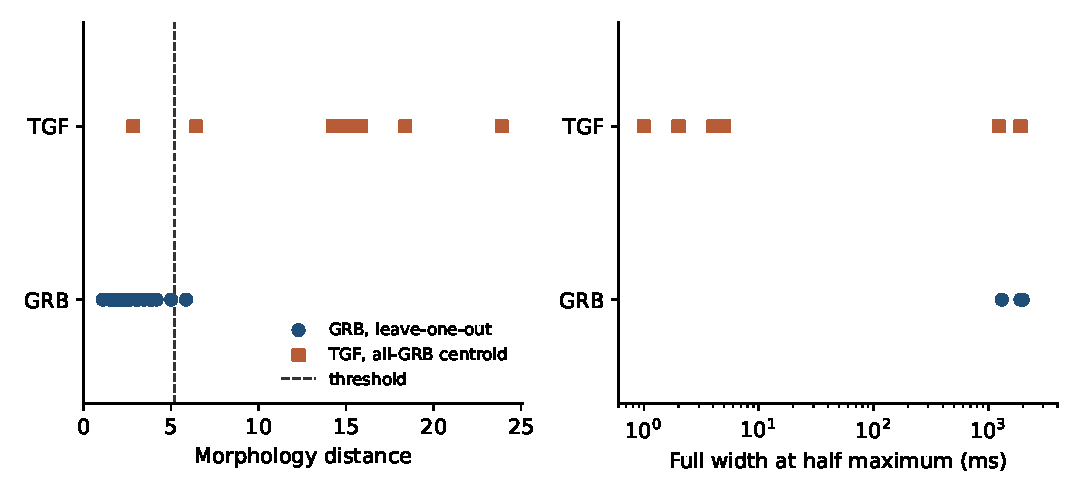
\includegraphics[width=0.92\textwidth]{fig_tte.pdf}
\caption{Morphology on 1\,ms TTE for the published GRB and TGF names. Left: distance to the GRB centroid. Bursts are leave-one-out. Flashes use the centroid of all 25 bursts. The dashed line is the 95th percentile of the burst distances, times $1.25$. Right: full width at half maximum of the background-subtracted sum, on a logarithmic axis.}
\label{fig:tte}
\end{figure}

\subsection{Lookup against a labeled fusion}
\label{sec:fusion}

The lookup is a table. Table~\ref{tab:fusion} asks what a learned combiner does with the same four numbers. The combiner is a class-weighted softmax on the physics residual, the morphology residual, $\log_{10}$ of the checksum, and the drop gain. The logarithm is a monotone rescaling: the raw checksum spans about eight decades, and a linear model standardized on that raw value cannot see a separation that a threshold can see. Training uses a disjoint simulator stream and includes flashes labeled novel. The lookup's thresholds are still fit on clean known-class residuals only. Both are scored on the published evaluation stream.

On single faults the fusion is the more accurate rule: $96.5 \pm 0.3\%$ four-way accuracy against $\AriaAcc\%$, sensor isolation $96.7 \pm 0.7\%$ against $\SensorIso\%$, and no held-out flash called compute. Compute isolation is $98.6\%$ on every seed, against $100\%$ for the lookup. The fusion does not turn a bit-flip into a discovery. On the 80 compound trials it does drop the checksum-first priority. It returns sensor on $72.5 \pm 7.5\%$ of them and compute on $27.5 \pm 7.5\%$, and novel on none. The lookup returns compute on all of them, including the trials whose sensor bit is also true. The accuracy belongs to the fusion, which was allowed to see the four labels. The refusal to preserve a corrupt product belongs to the lookup.

\begin{table}[t]
\caption{Lookup against a labeled fusion of the same four residuals on the simulator (percent, mean $\pm$ standard deviation over five training seeds). The fusion is a class-weighted softmax on the physics residual, the morphology residual, $\log_{10}$ of the checksum, and the drop gain. It is trained on a disjoint stream that includes flashes labeled novel. The lookup never receives those labels. Compound rows are the 80 spike-plus-bit-flip trials. The lookup column is the decision, so a compound trial whose sensor bit is also true is still counted as compute.}
\label{tab:fusion}
\centering
\small
\begin{tabular}{lcc}
\toprule
Metric & Lookup & Fusion \\
\midrule
Four-way accuracy & $90.0 \pm 0.6$ & $96.5 \pm 0.3$ \\
Novel isolation & $95.0 \pm 3.2$ & 100 \\
Novel $\to$ compute & $5.0 \pm 3.2$ & 0 \\
Compute isolation & 100 & 98.6 \\
Sensor isolation & $77.5 \pm 0.6$ & $96.7 \pm 0.7$ \\
Compound $\to$ compute & 100 & $27.5 \pm 7.5$ \\
Compound $\to$ sensor & 0 & $72.5 \pm 7.5$ \\
Compound $\to$ novel & 0 & 0 \\
\bottomrule
\end{tabular}
\end{table}


\section{Discussion}

The dictionary does what it was built to do on the simulator. A held-out TGF is usually called novel, a critical or protocol-mild bit-flip is called compute, a single-detector spike is called a sensor fault more often than not, and the three OOD-style baselines cannot make those distinctions. The ablations in Table~\ref{tab:abl} are the evidence that the distinction is the combination of residuals, not any one of them. The comparison in Table~\ref{tab:compare} is the evidence that this combination is not already a row in the literature. ProGIP is the nearest neighbor and still has no sensor symbol and no physics residual~\cite{progip2025}. Gertler's parity equations are the nearest structural neighbor and have no symbol for a new class~\cite{gertler1990}.

The same dictionary, on public CTIME, keeps the compute symbol and loses the novel symbol. That split is useful. It says the checksum does not need the simulator's light curves, and the morphology residual does, at 64\,ms. Figure~\ref{fig:morph} is the mechanism on those bins: TGF is not in the tail of the known-class distribution, and Figure~\ref{fig:sweep} says a lower threshold is not the remedy. Section~\ref{sec:tte} separates the two 1\,ms statements. Against a GRB-only centroid, 23 of 24 flashes sit beyond a threshold that 1 of 25 bursts also crosses. The four-way lookup, trained on bursts, flares, and magnetar bursts, names every flash a sensor fault. The physics residual is already above its ceiling, so the morphology bit is never consulted for those flashes, and Table~\ref{tab:ttelookup} shows that 8, 16, and 50\,ms bins keep that call. The discovery symbol on these files is a distance to one class. The lookup's call is sensor. At $12$ triggers per class the calibrated checksum names $8.3\%$ of CTIME flashes a compute fault, and the rounding bound removes those calls (Table~\ref{tab:realmodes}).

Sensor isolation is the weak single-fault cell, and the second download changes how the $60\%$ should be quoted. It is the rate on a GRB-heavy prefix when the physics threshold is sitting on its floor of $0.38$ (Table~\ref{tab:family}). A short-window template does not move it (Table~\ref{tab:spike}). A second draw, whose clean residuals push the same threshold to its ceiling of $0.62$, drops sensor isolation to $25\%$ in-sample and $7.5\%$ when that head scores the original slice (Table~\ref{tab:draw}). The quantity that travels is compute isolation.

The rounding bound is the one place a guarantee replaced a percentile, and it should be read as such. It was designed after the leak was observed. Its constant was not fit on injected faults, the fault-free ratio stayed below $1$ out to $1000$ standard deviations, and at binary32 it removed every false compute call in the simulator while keeping the protocol's flips. At binary16 it gives back most mild flips. A deployment that needs the guarantee has to pay that sensitivity, or it has to stay at binary32.

Compound faults are reported rather than hidden. The headline rule names them compute because the checksum is first, which is the safe operational error if the alternative is to preserve a corrupt product as a discovery. On $\BothSig\%$ of simulator compound trials the sensor bit is also true, so a deployment can refuse a single label. On the remaining $\ArithOnly\%$ the spike was invisible and no rule in this dictionary can recover it.

The fusion comparison narrows what the lookup is for. Given the four labels, a softmax on the same residuals is more accurate on single faults and still does not call a bit-flip a discovery (Table~\ref{tab:fusion}). It loses the property the table was built to keep: on a spike plus a bit-flip it usually returns sensor. Checksum-first is an operational choice, and Section~\ref{sec:fusion} is the measurement of what that choice costs.

What this paper does not establish is equally specific. It does not establish that the linear head's checksum catches a fault inside the convolutional-recurrent classifier of John and colleagues~\cite{john2025}. It does not establish a beam-test cross section. It does not run a streaming diagnostic monitor. Martingale tests that name the cause of a distribution shift already exist and are not used here~\cite{hindy2025}. It does run the four-way lookup at 1, 8, 16, and 50\,ms (Table~\ref{tab:ttelookup}). The novel symbol stays empty because the physics residual saturates. It does not establish that a Poisson matched filter on the real NaI response would change that call. It does not establish that real single-detector particle events in the catalog are the spikes injected here. Those catalog rows were counted and not classified.

\section{Conclusions}

OOD monitors and SDC monitors can say that an inference looks wrong. They cannot, by construction, say which of four operationally opposite causes produced that look when those causes share an activation-magnitude symptom. ARIA is a four-symbol isolability lookup whose residuals are forbidden from seeing the wrong cause. On a public-catalog-prior, GPU-free GBM-like simulator it separates held-out TGF from compute faults in most trials, names many sensor spikes, and fails honestly when two faults arrive together. A rounding-error bound removes the finite-precision leak that otherwise calls some TGFs a compute fault, at a sensitivity cost that appears at binary16. On \RealCubes{} real public CTIME triggers, compute isolation on critical and protocol-mild flips stays high, a held-out TGF is almost never named compute, and the discovery symbol does not survive at 64\,ms. A second disjoint draw keeps the compute symbol and the empty novel symbol, and it shows that sensor isolation is an artifact of where the clipped physics threshold sits. The same triggers at 1\,ms put 23 of 24 flashes outside a burst-only morphology. The lookup on the four-family download calls those flashes sensor, and coarser bins through 50\,ms keep that call. A labeled fusion of the residuals is more accurate than the lookup on single faults and names a compound fault as a sensor fault. The lookup is the rule that refuses that trade. The primitives, detector-to-detector vetoes, checksums, and centroid distance, are known. The dictionary that includes discovery as a non-fault symbol is the object of this work.

\section*{CRediT authorship contribution statement}

\textbf{Haripriya S.:} Conceptualization, Methodology, Software, Validation, Formal analysis, Investigation, Data curation, Writing -- original draft, Writing -- review and editing, Visualization. \textbf{Suhasini S.:} Supervision, Writing -- review and editing.

\section*{Declaration of competing interest}

The authors declare that they have no known competing financial interests or personal relationships that could have appeared to influence the work reported in this paper.

\section*{Funding}

This research did not receive any specific grant from funding agencies in the public, commercial, or not-for-profit sectors.

\section*{Declaration of generative AI and AI-assisted technologies in the writing process}

During the preparation of this work the authors used a large language model to assist with organization of the manuscript and with LaTeX formatting. After using this tool, the authors reviewed and edited the content as needed and take full responsibility for the content of the publication.

\section*{Data availability}

\begin{sloppypar}
HEASARC \texttt{fermigtrig}, Fermi-GBM CTIME, and time-tagged event files are public.
The cubes are \texttt{cubes.jsonl}, \texttt{cubes\_draw2.jsonl}, \texttt{tte\_cubes\_grb\_tgf.jsonl}, and \texttt{tte\_cubes.jsonl}, all under \texttt{experiments/gbm/}.
The burst-only distance uses the 24-flash file. The lookup uses the four-family file.
Regenerate with \texttt{npm run test:paper}, \texttt{npm run test:gbm}, \texttt{npm run test:gbm:heldout}, \texttt{npm run test:fusion}, \texttt{npx tsx src/lib/aria/score\_tte.ts}, \texttt{npx tsx src/lib/aria/tte\_lookup.ts}, and \texttt{npx tsx src/lib/aria/tte\_rebin.ts}.
\end{sloppypar}

\section*{Ethics statement}

The work uses public spacecraft triggers and a simulator. It involves no human participants, no animals, and no identifiable personal data.

\bibliographystyle{elsarticle-num}
\begin{thebibliography}{48}

\bibitem{meegan2009} C.~Meegan \textit{et al.}, The Fermi Gamma-ray Burst Monitor, Astrophys. J. 702 (2009) 791--804. \url{https://doi.org/10.1088/0004-637X/702/1/791}.

\bibitem{vonkienlin2020} A.~von Kienlin \textit{et al.}, The fourth Fermi-GBM gamma-ray burst catalog: a decade of data, Astrophys. J. 893 (2020) 46. \url{https://doi.org/10.3847/1538-4357/ab7a18}.

\bibitem{bhat2016} P.~N.~Bhat \textit{et al.}, The third Fermi GBM gamma-ray burst catalog: the first six years, Astrophys. J. Suppl. Ser. 223 (2016) 28. \url{https://doi.org/10.3847/0067-0049/223/2/28}.

\bibitem{poolakkil2021} S.~Poolakkil \textit{et al.}, The Fermi-GBM gamma-ray burst spectral catalog: 10 yr of data, Astrophys. J. 913 (2021) 60. \url{https://doi.org/10.3847/1538-4357/abf24d}.

\bibitem{roberts2018} O.~J.~Roberts \textit{et al.}, The first Fermi-GBM terrestrial gamma ray flash catalog, J. Geophys. Res. Space Phys. 123 (2018) 4381--4401. \url{https://doi.org/10.1029/2017JA024837}.

\bibitem{briggs2013} M.~S.~Briggs \textit{et al.}, Terrestrial gamma-ray flashes in the Fermi era: improved observations and analysis methods, J. Geophys. Res. Space Phys. 118 (2013) 3805--3830. \url{https://doi.org/10.1002/jgra.50205}.

\bibitem{paciesas2012} W.~S.~Paciesas \textit{et al.}, The Fermi GBM gamma-ray burst catalog: the first two years, Astrophys. J. Suppl. Ser. 199 (2012) 18. \url{https://doi.org/10.1088/0067-0049/199/1/18}.

\bibitem{goldstein2020} A.~Goldstein \textit{et al.}, Evaluation of automated Fermi GBM localizations of gamma-ray bursts, Astrophys. J. 895 (2020) 40. \url{https://doi.org/10.3847/1538-4357/ab8bdb}.

\bibitem{goldstein2019} A.~Goldstein \textit{et al.}, Updates to the Fermi-GBM targeted sub-threshold search in preparation for the third observing run of LIGO/Virgo, arXiv:1903.12597, 2019.

\bibitem{connaughton2015} V.~Connaughton \textit{et al.}, Localization of gamma-ray bursts using the Fermi Gamma-Ray Burst Monitor, Astrophys. J. Suppl. Ser. 216 (2015) 32. \url{https://doi.org/10.1088/0067-0049/216/2/32}.

\bibitem{kouveliotou1993} C.~Kouveliotou \textit{et al.}, Identification of two classes of gamma-ray bursts, Astrophys. J. 413 (1993) L101--L104. \url{https://doi.org/10.1086/186969}.

\bibitem{perera2025} A.~Perera, B.~Zackay, T.~Venumadhav, A new search pipeline for short gamma-ray bursts in Fermi/GBM data --- a 50\% increase in the number of detections, Astrophys. J. Suppl. Ser. 281 (2025) 4. \url{https://doi.org/10.3847/1538-4365/ae0189}.

\bibitem{john2025} A.~A.~John \textit{et al.}, Multivariate time series classification of Fermi-detected gamma-ray transients using convolutional-recurrent neural networks, Mach. Learn.: Sci. Technol. 7 (2026) 025046. \url{https://doi.org/10.1088/2632-2153/ae5501}.

\bibitem{bulgarelli2025} A.~Bulgarelli \textit{et al.}, Onboard machine learning for high-energy observatories for spacecraft autonomy and ground segment operations, Particles 8 (2025) 102. \url{https://doi.org/10.3390/particles8040102}.

\bibitem{hendrycks2017} D.~Hendrycks, K.~Gimpel, A baseline for detecting misclassified and out-of-distribution examples in neural networks, in: International Conference on Learning Representations, 2017.

\bibitem{liu2020} W.~Liu, X.~Wang, J.~D.~Owens, Y.~Li, Energy-based out-of-distribution detection, in: Advances in Neural Information Processing Systems, 2020.

\bibitem{liang2018} S.~Liang, Y.~Li, R.~Srikant, Enhancing the reliability of out-of-distribution image detection in neural networks, in: International Conference on Learning Representations, 2018.

\bibitem{lee2018} K.~Lee, K.~Lee, H.~Lee, J.~Shin, A simple unified framework for detecting out-of-distribution samples and adversarial attacks, in: Advances in Neural Information Processing Systems, 2018.

\bibitem{hsu2020} Y.-C.~Hsu, Y.~Shen, H.~Jin, Z.~Kira, Generalized ODIN: detecting out-of-distribution image without learning from out-of-distribution data, in: IEEE/CVF Conference on Computer Vision and Pattern Recognition, 2020, pp. 10951--10960.

\bibitem{wang2022} H.~Wang, Z.~Li, L.~Feng, W.~Zhang, ViM: out-of-distribution with virtual-logit matching, in: IEEE/CVF Conference on Computer Vision and Pattern Recognition, 2022, pp. 4921--4930.

\bibitem{bendale2016} A.~Bendale, T.~E.~Boult, Towards open set deep networks, in: IEEE Conference on Computer Vision and Pattern Recognition, 2016, pp. 1563--1572.

\bibitem{scheirer2013} W.~J.~Scheirer, A.~de Rezende Rocha, A.~Sapkota, T.~E.~Boult, Toward open set recognition, IEEE Trans. Pattern Anal. Mach. Intell. 35 (2013) 1757--1772. \url{https://doi.org/10.1109/TPAMI.2012.256}.

\bibitem{geng2021} C.~Geng, S.-J.~Huang, S.~Chen, Recent advances in open set recognition: a survey, IEEE Trans. Pattern Anal. Mach. Intell. 43 (2021) 3614--3631.

\bibitem{vaze2022} S.~Vaze, K.~Han, A.~Vedaldi, A.~Zisserman, Open-set recognition: a good closed-set classifier is all you need?, in: International Conference on Learning Representations, 2022.

\bibitem{yang2022} J.~Yang \textit{et al.}, OpenOOD: benchmarking generalized out-of-distribution detection, in: Advances in Neural Information Processing Systems, Datasets and Benchmarks, 2022.

\bibitem{ruff2021} L.~Ruff \textit{et al.}, A unifying review of deep and shallow anomaly detection, Proc. IEEE 109 (2021) 756--795. \url{https://doi.org/10.1109/JPROC.2021.3052449}.

\bibitem{gavarini2022} G.~Gavarini, D.~Stucchi, A.~Ruospo, G.~Boracchi, E.~S\'{a}nchez, Open-set recognition: an inexpensive strategy to increase DNN reliability, in: IEEE International Symposium on On-Line Testing and Robust System Design, 2022, pp. 1--7. \url{https://doi.org/10.1109/IOLTS56730.2022.9897805}.

\bibitem{sirc2022} G.~Xia, C.-S.~Bouganis, Augmenting softmax information for selective classification with out-of-distribution data, in: Asian Conference on Computer Vision, 2022, pp. 664--680.

\bibitem{narasimhan2024} H.~Narasimhan \textit{et al.}, Plugin estimators for selective classification with out-of-distribution detection, in: International Conference on Learning Representations, 2024.

\bibitem{progip2025} S.~Joshi \textit{et al.}, ProGIP: protecting gradient-based input perturbation approaches for OOD detection from soft errors, ACM Trans. Embed. Comput. Syst. 24 (2025) 118. \url{https://doi.org/10.1145/3761796}.

\bibitem{react2021} Y.~Sun, C.~Guo, Y.~Li, ReAct: out-of-distribution detection with rectified activations, in: Advances in Neural Information Processing Systems, vol. 34, 2021.

\bibitem{drdna2024} D.~Ma \textit{et al.}, Dr.\ DNA: combating silent data corruptions in deep learning using distribution of neuron activations, in: ACM International Conference on Architectural Support for Programming Languages and Operating Systems, vol. 3, 2024, pp. 239--252.

\bibitem{geissler2023} F.~Geissler, S.~Qutub, M.~Paulitsch, K.~Pattabiraman, A low-cost strategic monitoring approach for scalable and interpretable error detection in deep neural networks, in: Computer Safety, Reliability, and Security (SAFECOMP), Lecture Notes in Computer Science, vol. 14181, Springer, 2023, pp. 75--88.

\bibitem{schorn2020} C.~Schorn, L.~Gauerhof, FACER: a universal framework for detecting anomalous operation of deep neural networks, in: IEEE International Conference on Intelligent Transportation Systems, 2020, pp. 1--6.

\bibitem{blink2026} M.~Khan, A.~Malhotra, S.~K.~Gupta, BLINK: batch normalization-based integrity checkpoints for in-situ detection and mitigation of diverse weight corruptions in DNN accelerators, arXiv:2609.06781, 2026.

\bibitem{li2017} G.~Li \textit{et al.}, Understanding error propagation in deep learning neural network (DNN) accelerators and applications, in: International Conference for High Performance Computing, Networking, Storage and Analysis, 2017. \url{https://doi.org/10.1145/3126908.3126964}.

\bibitem{reagen2018} B.~Reagen \textit{et al.}, Ares: a framework for quantifying the resilience of deep neural networks, in: Design Automation Conference, 2018.

\bibitem{pytorchfi2020} A.~Mahmoud \textit{et al.}, PyTorchFI: a runtime perturbation tool for DNNs, in: IEEE/IFIP International Conference on Dependable Systems and Networks Workshops, 2020.

\bibitem{dixit2021} H.~D.~Dixit \textit{et al.}, Silent data corruptions at scale, arXiv:2102.11245, 2021.

\bibitem{hochschild2021} P.~H.~Hochschild \textit{et al.}, Cores that don't count, in: Workshop on Hot Topics in Operating Systems, 2021, pp. 9--16.

\bibitem{dixit2022} H.~D.~Dixit \textit{et al.}, Detecting silent data corruptions in the wild, arXiv:2203.08989, 2022.

\bibitem{gertler1990} J.~Gertler, D.~Singer, A new structural framework for parity equation-based failure detection and isolation, Automatica 26 (1990) 381--388.

\bibitem{venkatasubramanian2003} V.~Venkatasubramanian, R.~Rengaswamy, K.~Yin, S.~N.~Kavuri, A review of process fault detection and diagnosis. Part I: quantitative model-based methods, Comput. Chem. Eng. 27 (2003) 293--311. \url{https://doi.org/10.1016/S0098-1354(02)00160-6}.

\bibitem{isermann2005} R.~Isermann, Model-based fault-detection and diagnosis --- status and applications, Annu. Rev. Control 29 (2005) 71--85. \url{https://doi.org/10.1016/j.arcontrol.2004.12.002}.

\bibitem{chen1999} J.~Chen, R.~J.~Patton, Robust Model-Based Fault Diagnosis for Dynamic Systems, Kluwer Academic Publishers, 1999.

\bibitem{huang1984} K.-H.~Huang, J.~A.~Abraham, Algorithm-based fault tolerance for matrix operations, IEEE Trans. Comput. C-33 (1984) 518--528.

\bibitem{zhao2021} K.~Zhao \textit{et al.}, FT-CNN: algorithm-based fault tolerance for convolutional neural networks, IEEE Trans. Parallel Distrib. Syst. 32 (2021) 1677--1689. \url{https://doi.org/10.1109/TPDS.2020.3043449}.

\bibitem{kosaian2021} J.~Kosaian, K.~V.~Rashmi, Arithmetic-intensity-guided fault tolerance for neural network inference on GPUs, in: International Conference for High Performance Computing, Networking, Storage and Analysis, 2021.

\bibitem{approxabft2023} X.~Xue \textit{et al.}, ApproxABFT: approximate algorithm-based fault tolerance for vision transformers, arXiv:2302.10469, 2023.

\bibitem{higham2002} N.~J.~Higham, Accuracy and Stability of Numerical Algorithms, 2nd ed., SIAM, 2002.

\bibitem{ieee754} IEEE, IEEE Standard for Floating-Point Arithmetic, IEEE Std 754-2019, 2019.

\bibitem{hindy2025} A.~Hindy \textit{et al.}, Diagnostic runtime monitoring with martingales, in: Robotics: Science and Systems, 2025, arXiv:2407.21748.

\end{thebibliography}

\end{document}
